 \documentclass[11pt,a4paper]{report}
\usepackage[latin1]{inputenc}
\usepackage{csquotes}
\usepackage{amsmath}
\usepackage{mathtools}
\usepackage{pifont}
\usepackage{graphicx}
\usepackage{amsfonts}
\usepackage{amssymb}
\usepackage{fancyhdr}
\usepackage[left=4.5cm,right=4.5cm,top=4cm,bottom=2cm]{geometry}
\usepackage{listings}
\usepackage{color}
\usepackage{microtype}
\usepackage{booktabs}
\usepackage{chngcntr}
\usepackage{titlesec}
\usepackage{tikz}
\usepackage{float}
\usepackage{multicol}
\usepackage{tikz-qtree}
\usepackage{pgftree}
\usepackage{caption}
\usepackage{subcaption}
\usepackage{algorithm}
\usepackage{algpseudocode}
\usepackage[export]{adjustbox}
\usepackage[final]{pdfpages}
\usepackage{float}
\usepackage{caption}
\usepackage[square,sort,comma,numbers]{natbib}
\usepackage[super,negative]{nth}

                  
\usetikzlibrary{arrows, automata}

\setcounter{secnumdepth}{5}
\setcounter{tocdepth}{5}

\newcommand{\quotes}[1]{``#1''}
\newcommand{\at}{\makeatletter @\makeatother}
\newcommand{\HRule}{\rule{\linewidth}{0.5mm}} 
\pagestyle{fancy}%
  \renewcommand{\headrulewidth}{0.3pt}
  \renewcommand{\footrulewidth}{0pt}
  \renewcommand{\chaptermark}[1]{\markboth{#1}{}}
  \renewcommand{\sectionmark}[1]{\markright{#1}{}}
  \fancyhf{}
  \fancyhead[LE,RO]{\sffamily\bfseries\thepage}
  \fancyhead[LO]{\sffamily\bfseries\rightmark}
  \fancyhead[RE]{\sffamily\bfseries\leftmark}
  \fancyfoot{}
\renewcommand*\thesection{\arabic{section}}  

%\setcounter{secnumdepth}{5}
\counterwithin{paragraph}{subsubsection}
\counterwithin{subparagraph}{paragraph}


\begin{document}

\pagenumbering{Roman} 

\begin{titlepage}
\begin{center}
% Upper part of the page
%\LARGE Uppsala University \\[1.5cm]
%\textsc{\Large Thesis Specification}\\[0.5cm]
% Title
%\HRule \\[0.4cm]
{ \huge \bfseries \textbf{ Evaluating the performance of a new aligner for ultra-short ancient DNA }}\\[0.4cm]
\HRule \\[0.5cm]
% Author and supervisor
\begin{minipage}{0.9\textwidth}
\begin{flushleft} \large
{\textbf{Homa Amini}}\\
% Homa.Amini.0062\at student.uu.se\\
\end{flushleft}
\end{minipage}
%\begin{minipage}{0.4\textwidth}
%\begin{flushright} \large
%\emph{Supervisor:\\Janet Kelso}\\
%kelso\at eva.mpg.de
%\end{flushright}
%\end{minipage}
\vfill
% Bottom of the page
%{Create: \large Oct 2015}\\
%{Last update: \large \today}
\end{center}
\end{titlepage}

\newpage\null\thispagestyle{empty}\newpage
\newpage
\newpage

\section*{Abstract}

Recent technological developments, such as high-throughput sequencing,
have enabled the sequencing of the genomes of many living organisms.  Recently, it has also become possible to extract and sequence DNA from extinct organisms.\\ 
In comparison with modern DNA, the computational analysis of ancient DNA is complicated
by the fact that the sequenced fragments tend to be short, degraded and contaminated with
extraneous environmental sequences, such as bacteria and modern human DNA.

Identification of endogenous sequences from this mix of DNA is generally achieved by alignment to a reference genome sequence. 
However existing alignment software does not work well with these ultra-short, chemically damaged sequences.

In order to deal with these much older samples a new software program has been implemented
(R-Candy; U. Stenzel unpubl.)which aims to align these ultra-short reads and cope with the high 
levels of chemical damage present, using self-index data structures for pattern matching
based on a Burrows-Wheeler Transform based FM-Index.
%It supports genomes of any size and requires just ??? GB of memory.
It supports genomes of any size and requires not more than the provided genome size of memory.

This thesis evaluates the performance of the R-Candy aligner, using simulated data.

Tests on simulated datasets showed that R-Candy is the most accurate aligner currently available for ancient DNA sequences.

R-Candy yields a higher rate of sensitivity 
%(the number of correctly mapped endogenous genomic reads divided by the total number of endogenous reads)
and a low rate of false positive
% (the number of aligned microbial reads divided by the total number of microbial reads).
The current version of R-Candy compare to other aligners does not have a good throughput rate due to non-supporting multithreading feature. 

\newpage\null\thispagestyle{empty}\newpage
\section*{Acknowledgements}
\newpage\null\thispagestyle{empty}\newpage

\tableofcontents
\newpage
\listoftables
\newpage
\listoffigures
\newpage

\pagenumbering{arabic} 



\section{Introduction}


There have been a number of breakthroughs in the development of sequencing technologies that allow us to now sequence whole genomes rapidly and at a reasonable cost\cite{NGS}\cite{454}\cite{NGS2}.
\\
These developments made it possible to get DNA from ancient organisms, including humans \cite{AncientDNA}\cite{fish2human}, and to sequence this DNA to learn about human history\cite{impactOFhg}\cite{ourGenome}\cite{SNP}.

Since the primary goal of many studies is to find the genetic relationships between extinct and extant species, 
most often sequences from ancient organisms are analysed by aligning them to the genomes of closely related extant species\cite{Neanthertal}\cite{AncientDNA}.

A number of problems have to be addressed when ancient DNA is aligned.
The continuous maintenance of a living organism by enzymatic repair stops shortly 
after a death of a living organism. Along with the aggression of microbes,
insects and fungi on the DNA molecule make the extraction of a high-quality 
endogenous DNA of the original owner(not the contaminant sources of DNA) 
very difficult and result in very short(the mean aDNA fragments vary between 
36 to 150 base pairs providing by Illumina platform\cite{rizzi2012ancient} 
\footnote{This range varies due to environment and the age of the sample})
 and degraded DNA sequences\cite{paabo2004genetic}.
In addition to \emph{post-mortem} damage which is the degradation process of
ancient DNA over time results in deamination of cytosine to uracil and C to T 
changes at the both ends of DNA fragments \cite{futureofaDNA}, the low amount 
of survived endogenous DNA over a long period of time (above 38,000 years) 
are highly contaminated \cite{paabo2004genetic}\cite{aDNA}.

As mentioned before there are two sources of contamination in ancient DNA.
First microbial contamination (bacteria of colonized dead organisms) and second present-day human contamination that comes from the first touch in excavation sites and afterwards in the process of preparing PCR libraries in the sequencing laboratories \cite{AncientDNA}.

For samples that are reasonably preserved approaches to the alignment of reads that are longer than 35bp have been developed. 
These use standard alignment software (eg BWA) but modify the parameters to compensate more differences.
But for older or less well-preserved samples that have even shorter sequences $(<35 bp)$ \cite{meyer2014mitochondrial},
using standard aligners like BWA leads to spurious alignments for a number of reasons.

First given the mammalian genome size - random alignments of shorter sequences become increasingly likely as the length decreases. This means that an increasing number of incorrect alignments can be found (and this is true for both endogenous and microbial DNA).

Second, standard aligners don't include a model of chemical damage that is specific to ancient DNA, and, therefore, penalise reads with mismatches that are due to chemical damage.

Third, most aligners require an exact match of some minimum length(seed), that is often longer than the read length possible with ancient DNA.

Fourth, the ultra-short sequence fragments with some 
substitution regarding mutation, divergence,  sequencing error and \emph{post-mortem} damage are so likely to be found alignments with an exact match while the original location of 
the read is reachable with some mismatches.

Fifth, aligning short reads to a genome with a lot of repetitive elements which often are longer that the length of the reads needs a sensitive heuristic method that gives the higher probability to the original location over the other locations.

Therefore, due to the lack of proper tools such as an aligner that is specific to ancient data and its characteristics, most of the generated data get discarded. 
This information reduction on the datasets of sparce endogenous data give us the motivation for 
a new aligner to efficiently analyze this particular type of data.
\\
The alignment of ancient DNA reads with high accuracy to the reference genome is a crucial step in application workflows such as ancient DNA pipeline, contaminations estimation, divergence estimation, genotyping, heterozygous estimation, etc
\\
A number of aligners have been developed to undertake this task such as BWA\cite{bwa} and BWA-PSSM\cite{pssm}.
Each aligner provides different trade-offs between mapping accuracy and speed. 
For example, different parameters that compromised the mapping accuracy to reduce runtime are\cite{benchmarking}:\\
Limiting the number of allowed mismatches,
Limit the length of allowed gaps and
neglecting base quality score.
\\\\

In this thesis, I present a comparison between standard BWA, a modified version of BWA for working with ancient data and R-Candy.

The accuracy of these aligners is evaluated on different settings. 
%A read is defined to be correctly mapped if it maps to the correct location in the genome and has the best quality score(lower or equal to the threshold). 
I considered small simulated data sets of 700,000 reads of lengths 25, 30, 35 and 40 bps and map against a simulated genome of length 1Gbp and the Human genome of length 3Gbp as the reference genomes.

%Evaluating the sensitivity of the aligners according to the number of intervals they detected. The sensitivity evaluation criteria is used to evaluate the performance of both aligners on simulated and real genome.

% Additionally, the error model I use does not include INDELs and only allows mismatches.

Two different sets of experiments are presented to evaluate and understand the strengths and weaknesses of the new aligner(r-candy).

The first set includes the benchmarking suite, consisting of tests that cover input properties and algorithmic features. These tests are applied to genomic and microbial resequencing synthetic data to verify the effectiveness of the benchmarking tests. 

We consider a read alignment correct if the read is aligned to its original location in the genome and has the best alignment score(lower or equal to the threshold)
Although it is biologically relevant but has some computational pitfalls. For example, a read can be aligned to its original genomic location with some mismatches (due to sequencing error or other substitutions called SNP) while there is an exact match to another location. Therefore, an aligner needs another criterion to take the inexact match but the right location over the exact match. 

Unlike the BWA,  R-Candy reports all the mapping locations of a read, therefore,  
in order to compare the mapping accuracy performance of the two aligners, in the case of multiple alignments for r-candy we chose one alignment arbitrarily over the others, even though comparing the execution time performance will not be fair.  

I also emphasize on the effect of the indexing technique on the performance of the R-Candy which the

BWA also uses a Burrows-Wheeler transform based FM-Index but with different axillary data structures.



\subsection{Terminologies}

\begin{itemize} 
	\item  \emph{DNA }: or deoxyribonucleic acid is a hereditary long molecule in human and all other organisms that contains the genetic information needed for development and reproduction of living organisms.
	
	
	\item \emph{Nucleotide}: DNA contains four basic building blocks or bases: Adenine, Cytosine, Thymine and Guanine denoted by A, C, T and G respectively.The order of these nucleotides determine the instruction of a DNA molecule.
	
	\item DNA is a two-stranded double helix shape molecule where nucleotides in each strand pair together with the complementary nucleotide (A with T, C with G) on the opposite strand. Two strands run on anti-parallel in the way that on runs on \enquote*{5} to \enquote*{3} (The beginning and end of each strand respectively) and the other one runs \enquote*{3} to \enquote*{5}.
	
	\item \emph{Next-generation sequencing technology (NGS)}: also known as massively parallel sequencing.
	Includes technologies such as: Illumina, SOLiD, 454 which was a very important technology in early days and then Pacific Bioscience (PacBio).
	
	%\item \emph{First generation sequencing technology}: Basically refers to Sanger sequencing.
	
\end{itemize}

\subsection{Ancient DNA }
The ancient DNA exploration broadly describes as the retrieval of DNA sequences from fossils remains, archaeological discovery, museum specimens and other exceptional sources, only become doable when the new technologies for amplification and sequencing of DNA sequences, called PCR got invented \cite{paabo2004genetic}.

The extracted DNA from long-dead organisms has significantly different characteristics that differ it from modern DNA which are summarized in Table\ref{aDNAchar} .\\



\begin{table}[H]
  \begin{tabular}{ |  p{4cm} | p{2cm} | p{5cm} |}
    \hline
  \textbf{  Properties} & \textbf{Modern DNA } &\textbf{ ancient DNA} \\ \hline
       Length &  100 bps  & $\leq$  35 bps \\ \hline
       Post-Morten substitutions & No  & Deamination of C$\to$T
(more likely near the end of a read) \\ \hline
  Contaminated & negligible & Microbial+Modern human\\ \hline
    \end{tabular}
\caption{Comparison between modern DNA and ancient DNA}
\label{aDNAchar}
\end{table}

%\textbf{Length:}The continuous maintenance of a living organism by enzymatic repair stops shortly after a death of a living organism. Along with the aggression of microbes, insects and fungi on the DNA molecule make the extraction of a high-quality endogenous DNA of the original owner(not the contaminant sources of DNA) very difficult and result in very short(the mean aDNA fragments vary between 35 to 150 base pairs providing by Illumina platform\cite{rizzi2012ancient}) and degraded DNA sequences\cite{paabo2004genetic}.\\\\
%\textbf{Post-Mortem damage:} the degradation of DNA molecule to small average size (the mean aDNA fragments vary between 35 to 150 base pairs providing by Illumina platform\cite{rizzi2012ancient}) by enzymes shortly after death as well as feeding of bacteria, fungi and insects on organisms after their death\cite{paabo2004genetic}.
%\textbf{Post-Mortem damage:} 
%The degradation process of ancient DNA over time results in deamination of cytosine to uracil and C to T changes at the both ends of DNA fragments \cite{futureofaDNA}.\\\\
%Therefore, the low amount of survived endogenous DNA over a long period of time (above 38,000 years) are highly contaminated \cite{paabo2004genetic}\cite{aDNA}.\\\\
%\textbf{Contamination:}
%There are two sources of contamination in ancient DNA.
%First microbial contamination (bacteria of colonized dead organisms) and second present-day human contamination that comes from the first touch in excavation sites and afterwards in the process of preparing PCR libraries in the sequencing laboratories \cite{AncientDNA}.\\


The challenges with ancient DNA was the requirement for new software to efficiently 
align millions of ultra-short, degraded and deaminated reads to a reference genome.


\subsection{Alignment}
%Alignment or mapping of reads is determining the corresponding part of the reference sequence for each read in our sequence data.\\

%An alignment between two strings $S_{1}$ and $S_{2}$ aims to highlight the similarities between two sequences and reveals their relationship.\\
%This concept gets more interesting when a string $S_{1}$ changes into $S_{2}$ over time, through some operations like substitution/mutation of one character with/into another one or insertion or deletion of a character.\\

That sequence alignment is a common problem in computational biology, and one that can be simplified as follows:

An alignment between two strings $S_{1}$ and $S_{2}$ assumes a common origin and 
tries to highlight their similarities by explaining one of them as a small number 
of mutations, insertions and deletions applied to the other.\\

For those characters the survived over the times, an alignment of two strings is a list of indices (i,j) where $S_{1}[i]$ matches $S_{2}[j]$.\\ 
In its simplest form an alignment of two strings is obtained by placing two strings one above 
the other one in the way that every character in either string is above a unique character 
in opposite string and then looking for relation between them.\\\\
%(more details in the background on section 2.2)\\
As an example, consider the alignment of two strings $S_{1}$:\emph{'CCGATGA'} and $S_{2}$:\emph{'TCGCTG'} shown below. 

\begin{center}
	%\begin{tabular}{c *{12}c|cc|c}
	\begin{tabular}{ c c c |c| c c |c|c| c c|c| c c}
%	\hline
   $S_{1}$   &  & & C & C & G & A & - & T & G & A && \\
	%\hline
$S_{2}$ 	&  & &{\textcolor{red}T}& C & G & {\textcolor{green}-}& {\textcolor{cyan}C }  &  T & G & {\textcolor{green}- }& \\
    	                                 
	\end{tabular}
\end{center} 
In this alignment,there is one mismatch of character T highlighted in red, 
two deletion of character A highlighted in green and one insertion of character
C highlighted in cyan and all the other characters match their counterparts in the opposite string. 
\\\\

There are some key issues for an ideal alignment that needs to be considered:

\begin{itemize} 
	\item  What sort of alignment.
	\item  What kind of scoring system.
	\item  What algorithm to find the optimal alignment score.
\end{itemize}


\subsubsection{The Scoring Model}

Comparing two sequences, we need a score to measure their similarity.
In the case of biological, the assumption is that the two sequences differ
due to a mutation process that led to a substitution 
of one base by another base,as well as insertion and deletion (INDEL) which add or remove bases.
We are aiming at aligning the two sequences in a way that maximizes their similarity.\\ \\
First, let me set up the problem with some notation:\\
We call the two sequences, $S_{1}$ and $S_{2}$ of length N and M respectively. 
The $i^{th}$ symbol in $S_{1}$ is $S_{1i}$ and $j^{th}$ symbol in $S_{2}$ is $S_{2j}$. 
In the case of DNA, these symbols are $\left\{A, C, G, T\right\}$.\\
$S(S_{1i}, S_{2j})$ is the score of aligning $S_{1i}$ to $S_{2j}$ (match or mismatch)
and $\delta$ is a penalty for introducing a gap by insertion or deletion of a character. 
Then the score of an alignment will be the sum of the substitution scores minus the 
penalties in it(the scoring system for our alignment is described in section 3.2.1.5 in more details).\\\\
As an example, the following is the substitution matrix for DNA sequence alignments.


\begin{table}[H]
 \centering
  \begin{tabular}{  c| r  r r  r }
    
  \textbf{  $S(S_{1i}, S_{2j})$ } & \textbf{A} &\textbf{ C} &\textbf{ G} &\textbf{ T} \\ \hline
       \textbf{A} &  1  & -1 & -0.5 & -1 \\
       \textbf{C} & -1  & 1 & -1 & -0.5 \\ 
       \textbf{G} & -0.5 & -1 & 1 & -1 \\ 
       \textbf{T} & -1 & -0.5 & -1 & 1
    \end{tabular}
%\caption{comparation between modern DNA and ancient DNA}
\label{alignment-exp}
\end{table}

If $\delta$=1 then the total score of following alignment is:
 
\begin{center}
	\begin{tabular}{c *{12}cccc}
%	\hline
        & & C & C & G & A & - & T & A & G && \\
	%\hline
 	  & & T  & C & G &  -  & C   &  T & -  & G & \\
    	                                 
	\end{tabular}
\end{center} 

-0.5 + 1 + 1 - 1 - 1 + 1 - 1 + 1 = 0.5

\subsubsection{Alignment Algorithms}

Having the scoring system, we need an algorithm for finding the optimal alignment 
between a pair of sequences. Why we need a complicated heuristic algorithm and can
not just calculate the all possible alignments and choose the best one?\\
Because it is not computationally practical to calculate  
$$ \binom{2n}{n} = \frac{(2n)!}{(n!)^2} \simeq \frac{2^{2n}}{\sqrt{2\pi n}} $$
possible alignment between two sequences of length N. The problem gets even more complicated when we allow for gaps. 
The algorithm that guarantees to find the optimal alignment between a pair of sequences base on the best alignment 
score is an instance of dynamic programming. 
Dynamic programming has an essential role in computational sequence analysis.\\ 
For different types of alignment, there are slightly different types of dynamic programming algorithm(alignment algorithms).\\\\

The four essential steps in all dynamic programming algorithms are:

\begin{itemize} 
	\item Define a recursive structure for the optimal score\cite{eddydynamic}.
	\item  Create a  matrix for remembering the optimal score of subproblems \cite{eddydynamic}.	
	\item Fill the matrix by solving the  subproblems in a bottom-up approach\cite{eddydynamic}.
	\item Reconstruct the optimal approach that led us to the optimal score by a traceback on the matrix\cite{eddydynamic}.
\end{itemize}

In the following part I will describe the two more basic alignment algorithms that easily can be expanded to the more complex versions.

\paragraph{ Global alignment ( Needleman-Wunsch algorithm) }

The Needleman-Wunsch algorithm, which is based on dynamic programming is a widely used/well-known global alignment technique in biological sequence analyses to obtain the best-matching alignment of two sequences, allowing  gaps.\\
It aims to construct an optimal alignment using previous solutions for
optimal alignments of smaller subsequences \cite{durbin}.\\
We are going to calculate the optimal alignment score as been described in\cite{durbin} by constructing a matrix F indexed
by i and j, one index for each sequence, where the value F(i, j) is the score
of the best alignment between the initial segment $S-{1i..i}$ of $S_{1}$ up to $S_{1i}$ and the initial segment $S_{21..j}$ of $S_{2}$  up to $S_{2j}$. We can build F(i, j) recursively start by initialising F(0, 0) = 0. Afterwards we fill the matrix matrix from top left to bottom right. 
Once $ F(i-1, j-1 ), F(i-1 , j) $ and $ F(i , j-1) $ are known, we are able to calculate $ F(i, j)$ \cite{durbin}.

The best score of F(i,j) up to $S_{1i}$ and $S_{2j}$ is the maximum value of $S(i,j)$:

\[ F(i,j)= max
\begin{cases}
   F(i-1,j-1) + S(S_{1i} , S_{2j})\\
   F(i-1 , j)- \delta\\
   F(i,j-1)- \delta
\end{cases}
\]
The value in the last cell of matrix F(n,m) is by definition the optimal alignment score. 
For obtaining the alignment itself we need the path that led us to the final score. We use the traceback procedure to recursively recover the optimal alignment\cite{durbin}\cite{eddydynamic}.
We start from the last cell F(n,m) and follow each of the three cases that we chose to get to this point. We continue doing this until reaching the cell F(0,0) and in this point the optimal alignment is completely reconstructed \cite{eddydynamic}.



\paragraph{ Local alignment ( Smith-Waterman algorithm ) }

Compute the maximum scoring alignment of $L(S_{1}, S_{2})$ over all subsequences $S_{1}$ and $S_{2}$ is:


\[ F(i,j)= max
\begin{cases}
   F(i-1,j-1) + s(S_{1i} , S_{2j})\\
   F(i-1 , j)- \delta\\
   F(i,j-1)- \delta\\
   0 \quad  
\end{cases}
\]
The best way to understand how the local alignment algorithm works is to see an example.\\

We have two sequences and want to optimally align them.
$$S_{1}:ACACACTA$$
$$S_{2}:AGCACACA$$\\
$s(S_{1i},S_{2j})= +2 \quad if \quad S_{1i} = S_{2j}(match) \quad and \quad-1 if \quad S_{1i}\neq S_{2j}(mismatch)$\\



\[
H = 
 \begin{pmatrix}
   & $\_$ & A & C & A & C & A & C & T & A \\
 $\_$ & \textcolor{red}{0} & 0 & 0 & 0 & 0 & 0 & 0 & 0 & 0 \\
 A & 0 & \textcolor{red}{2} & 1 & 2 & 1 & 2 & 1 & 1 & 2 \\
 G & 0 & \textcolor{red}{1} & 1 & 1 & 1 & 1 & 1 & 0 & 1 \\
 C & 0 & 1 & \textcolor{red}{3} & 2 & 3 & 2 & 3 & 2 & 2 \\
 A & 0 & 2 & 2 & \textcolor{red}{5} & 4 & 5 & 4 & 4 & 4 \\
 C & 0 & 1 & 4 & 4 & \textcolor{red}{7}  & 6 & 7 & 6 & 6 \\
 A & 0 & 2 & 3 & 6 & 6 & \textcolor{red}{9} & 8 & 8 & 8 \\
 C & 0 & 1 & 4 & 5 & 8 & 8 & \textcolor{red}{11} & \textcolor{red}{10} & 10 \\
 A & 0 & 2 & 3 & 6 & 7 & 10 & 10 & 10 & \textcolor{red}{12} \\
  
 \end{pmatrix}
\]

After filling the matrix, the optimal alignment score will be the last score that we calculate.
But we still do not have the optimal alignment which will be recover by back tracing the path that led us to the final score.



\[
T = 
 \begin{pmatrix}
       & $\_$ & A & C & A & C & A & C & T & A \\
  $\_$ & \textcolor{red}{0} & 0 & 0 & 0 & 0 & 0 & 0 & 0 & 0 \\
 A & 0 & \textcolor{red}{\nwarrow} & \leftarrow & \nwarrow & \leftarrow & \nwarrow & \leftarrow & \leftarrow & \nwarrow \\
 G & 0 & \textcolor{red}{\uparrow} & \nwarrow & \uparrow & \nwarrow & \uparrow & \nwarrow & \nwarrow & \uparrow \\
 C & 0 & \uparrow & \textcolor{red}{\nwarrow} & \leftarrow & \nwarrow & \leftarrow & \nwarrow & \leftarrow & \leftarrow \\
 A & 0 & \nwarrow & \uparrow & \textcolor{red}{\nwarrow} & \leftarrow & \nwarrow & \leftarrow & \leftarrow & \nwarrow \\
 C & 0 & \uparrow & \nwarrow & \uparrow & \textcolor{red}{\nwarrow} & \leftarrow & \nwarrow & \leftarrow & \leftarrow \\
 A & 0 & \nwarrow & \uparrow & \nwarrow & \uparrow & \textcolor{red}{\nwarrow} & \leftarrow & \leftarrow & \nwarrow \\
 C & 0 & \uparrow & \nwarrow & \uparrow & \nwarrow & \leftarrow & \textcolor{red}{\nwarrow} & \textcolor{red}{\leftarrow} & \leftarrow \\
 A & 0 & \nwarrow & \uparrow & \nwarrow & \uparrow & \nwarrow & \uparrow & \nwarrow & \textcolor{red}{\nwarrow} \\
 \end{pmatrix}
\]

In the example, the last cell of the matrix (8,8) has the highest value. The trace back corresponds to the red path in the matrix, is the optimal alignment of the two sequences $S_{1}$ and $S_{2}$: 

$$S_{1}:A-CACACTA$$
$$S_{2}:AGCACAC-A$$



\paragraph{Semi-global alignment}

Semi-global or "global" (short for global-local) algorithm is a combination of global and local alignments. It is a practical strategy in some situations such as our case: aligning two sequences when one is short (for example an ancient sequence) and the other one is long(for example a chromosome sequence). In this case, neither global nor local alignment is completely applicable. The best solution here is to globally align the short sequence while only a local alignment is appropriate for the long sequence.

%\\\\\\\\
%\emph{\textbf{You have not mentioned classic alignment algorithms that have been used in the past, nor the idea that the aim is to minimise some kind of a score in order to find the most optimal alignment. Some literature review here would be useful.  There is a book called Biological Sequence Analysis  by Durbin and Eddy.  It might be useful. Even the wikipedia entry provides relevant background.} }
%https://en.wikipedia.org/wiki/Sequence_alignment 

%Mapping is alignment to a large, static genome and correspond to the offline approximate string matching problem. 

%%%%%%%%%%%%%%%%%%%%%%%%%%%%%%
%\subsection{Why a New Aligner is Required }
%\emph{\textbf{The three points below don't capture well the reasons shorter fragments are harder to align.}}\\\\

%As mentioned above, Ancient DNA has fragmented DNA molecules which can lead to shorter reads.
%These short reads are harder to align because:\\
%\begin{enumerate}
%\item Given the mammalian genome size - random alignments of shorter sequences become increasingly likely as the length decreases. This means that an increasing number of incorrect alignments can be found (and this is true for both endogenous and microbial DNA)\\
%\item Standard aligners don't include a model of chemical damage that is specific to ancient DNA, and therefore penalise reads with mismatches that are due to chemical damage.\\
%\item  Most aligners require an exact match of some minimum length, that is often longer than the read length possible with ancient DNA\\
%\item Damage creates the same problem; matches are not exact i.e. the heuristic needs
%to be able to allow for one or more mismatches while disentangle this from damage.\\
%\item Contamination increases the false-positive rate since it is hard to distinguish
%between incorrect matches (produced by contamination) and true-positive endogenous reads.\\\\
%\end{enumerate}



%%%%%%%%%%%%%%%%%%%%%%%
\subsection{Objectives}

The key motivation behind this thesis comes from the crucial needs for 
sophisticated computational tools and methods to deal with massive amount of ancient data coming from archeological remains such as teeth \cite{teeth}, bones \cite{hagelberg1989ancient}, hair \cite{gilbert2004population}, coprolites \cite{coprolites} and soft tissue.
% that needs new method and tool for new types of data.\\

In this thesis we aim to address this need by evaluating the performance of an ancient DNA specific aligner called R-Candy developed by Udo Stenzel at Max Planck institute that is optimized for ultra-short reads of length 30 to 50 with a high level of microbial contamination and extensive deamination using real and simulated data sets. \\


I show that alignments of such a data using existing heuristics (e.g. BWA) are not good enough for our purposes.\\ 

R-Candy has a novel scoring system that takes in account the deamination of C to T(replacement of cytosine with uracil) and G to A(opposite strand) that improves the accuracy and performance of a sequences alignments, as I will show in the result section. 

It is a Haskell based open source software(https://github.com/udo-stenzel/r-candy.git) which is specific for aligning ancient DNA sequences.



%%%%%%%%%%%%%%%%%%%%%%
\subsection{Structure of the Thesis}

\textcolor{violet}{\textbf{\emph{Check again at the end in case new sections have been included.}}}
\\\\
The thesis is organized as follow:
 
Section 2, I introduce some data structures like Suffix arrays and FM-Index for fast pattern matching. In addition Burrows-Wheeler transform, Wavelet tree and \emph{rank9} data structure will be introduced.

Section 3 will describe our approach to R-Candy aligner implementation.
I will provide an overview of different data structures used by R-Candy and its alignment algorithm and scoring system.

In Section 4, I will describe how we evaluated the performance of our aligner and present the result of applying R-Candy on simulated and real datasets in comparison with BWA aligner.

Finally, we will summarize our achievements in Section 5 and improvement of R-Candy's performance will be discussed in Section 6. 




\clearpage


\section{Background }

Determining the corresponding part of a genome for DNA sequences is a special case of pattern matching.
Where the incorporation of the special DNA characteristics and the sequencing technologies make it more challenging.
\\\\
Some features of DNA and sequencing technologies, which can influence the mapping process:
\begin{itemize} 
 \item \emph{Seeding}
The seeding feature that is used to to maximize performance and accuracy could simply be defined as follows:\\
Theorem: if a Pattern occurs in a genome with N mismatches, and divide the genome into N+1 equal pieces, at least, one piece has an exact match. 
Due to the properties of NGS technologies, the first few base pairs of a read sequence contains fewer errors. And the seed regions are supposed to have fewer false characters.

 \item \emph{The base quality score} is a measure of correctly reading each base in a read by a sequencing machine which is defined by the Phred score(for more explanation see Section 4.0.3.3 Sequencing Error ).
The quality scores can be used to determine mismatch locations.

% \item \emph{SNP}
%A single nucleotide polymorphism called SNP is a common type of genetic variations among  individuals of the same species. 
%SNPs could easily be mistaken as mismatches in the mapping process, where the true identification of their location before the mapping could improve the quality of mapping.


 \item \emph{Paired-end reads}
The \quotes{paired-end} expression refers to sequencing both ends of a DNA molecule.
It increases the mapping accuracy by having the distance information
 between the end points.
 
 \item \emph{INDELs existence}  which is allowing insertion or deletion of a nucleotide(base) while aligning a sequence to a reference string of a genome called gaps.Choosing the location of a gap gets so complicated regarding the length of a read especially in the case of ancient data where the read length is ultra-short(25-50 bps). Therefore, some aligners do not allow any gaps or limit their numbers and locations while dealing with short reads.
 
\end{itemize}

\subsection{Tools' Description}

The mapping procedure for most of the existing aligners (including R-Candy and BWA) starts by indexing the reference genome in order to accelerate the process of finding the corresponding position of each read in the reference.
One of the most common techniques to build an index for a reference genome or reads is Burrows-Wheeler Transform.
\\
In general Burrows-Wheeler Transform is an efficient data indexing technique that requires a small amount of memory while searching a query through a big data string(more details in Section 2.2.2).\\

To evaluate the performance of R-Candy, I tested an additional
alignment program called BWA.
BWA is a Burrows-Wheeler Transform based aligner that uses backward search (Ferragina and Manzini, 2000) 
to find matches  between a query and substring of the reference string within a certain defined distance\cite{bwa}.

Each aligner supports different sequencing technologies features and handles them differently apart from differences in their mapping approach.
For example, R-Candy uses an alignment score to accept or reject and alignment while BWA alignment technique for accepting or rejecting an alignment is based on the number of mismatches between the read and the reference genome\cite{bwa}.


\begin{table}[H]
 \centering
 \caption{features supported by tools}
  \begin{tabular}{ |  p{4cm} | c | c |}
   \hline 
  				  	   & \textbf{R-Candy} &\textbf{ BWA}  \\ \hline
  	   Post-mortem damage & Yes & - \\	  	   
       Seed mismatches &  -  & Any  \\
   Non-seed mismatches & AS  & Count  \\ 
          Gapped align & partially & partially \\ 
       Mapping quality & - & Yes  \\
       Var. seed len.  & -   &  Any \\
       \hline
      \end{tabular}
	\caption*{count: total count of mismatches in the read, AS: alignment score. 
	%Gap alignment for R-Candy is limited to 1 and for BWA is limited to .
	 }
 	\label{features}
\end{table}

%The mapping quality used by BWA is a Phred-scaled probability of the alignment being incorrect\cite{bwa}.
%While
%The R-Candy's alignment score is the probability of the occurrence of the read sequence given an alignment location.

\subsubsection{Default options of the tested tools}

Generally, using a tool with its default parameters gives a good performance. Most of the time users use the tools with the default setting or just tweak some of them. Thus, it is important to know these
options and the effect of using them.  
The most important default parameters of the two considered aligners in this thesis are the following:

\begin{itemize} 
 \item \emph{Alignment score}  which is the probability of the occurrence of the read sequence given an alignment location is set to 12 for R-Candy by default and BWA does not provide alignment score for its alignments.
 
 \item \emph{post-mortem damage deamination parameters:} For R-Candy the left and right overhang parameters which are used to calculate the length of overhangs by geometric distribution in 5' and 3' ends respectively are sets as zero in case the reads are not ancient and do not have \emph{post-mortem} damage.The deamination rates of cytosine residues into uracil residues for double and single stranded parts of a read are set by default 0.02 and 0.45 respectively.\\
BWA does not include \emph{post-mortem} damage at its alignment process.

 
 \item \emph{Divergence rate:} which is defined as one-third of the expected divergence rate between the reads and reference genome.  R-Candy's default divergence rate is 0.005,  assuming aligning a human genome to a chimpanzee genome.\\\
 Not available for BWA.
  
 %\item \emph{INDEL rate:}???
  
 \item \emph{Maximum number of allowed mismatches in the read:}  BWA determines the number of mismatches based on the read length. For 15-37 bps reads is 2; for 38-63 bps is 3; for 64-92 bps is 4, for 93-123 bps is 5 and for 124-156 bps is 6\cite{bwa}.
For R-Candy, it is included in its alignment score.

 \item \emph{Seed length and Maximum number of allowed mismatches in the seed:} By default, the seed length for BWA is 32 bps allowing maximum two mismatches in this part to speed up the alignment. But for reads shorter than seed region, BWA's seeding feature is disabled.
Generally, the seeding strategy needs long reads which in the case of ancient data is not achievable therefore R-Candy does not support seeding.
 
%Minimum and maximum insert sizes for paired-end mapping: The insert size represents the distance between the two ends. The values used for the minimum and the maximum insert size is 500 for BWA.

\end{itemize} 

Therefore, it's important to have the same values when comparing two pieces of software because different default values lead to different results for the same datasets.\\


\subsection{Evaluation criteria}
The performance of the aligners have been evaluated by three aspects, namely, 
operating characteristic (performance of a binary classifier system).
The performance of a binary classifier system is the true positive rate(sensitivity) and false positive rate(fall-out).
%the mapping percentage(?? what should I call the ROC curve), the throughput(or speed) and memory footprint.
%The mapping percentage is the percentage of aligned reads for each aligner.(should I mention FP rate as well ?)


The aligner's throughput is the number of mapped reads per second(bps/sec)
whereas the memory footprint is the required memory by the tool for indexing reference string, process the reads and storing them. 

The sensitivity reported is the number of correctly mapped 
endogenous genomic reads divided by the total  of simulated endogenous reads.\\ 
The fall-out is the number of aligned  microbial reads 
divided by the total number of  microbial reads.

The mapping sensitivity is divided into two parts, a correctly mapped reads (true positives) part and an error (false positives) part. 
There are different ways of calculating the error. For simulated reads,
 the percentage of reads mapped to the incorrect location (aligned to a position differ than the original position in the genome where the read was originally extracted from) which is a common definition of error used in many studies\cite{ErrorDef}. 

But, this na\"\i ve definition of the correctness of an alignment has some pitfalls. For example after applying sequencing error and \emph{post-mortem} damage(deamination) on the reads, the read does not exactly match the original genomic position. And it would be a problem for an aligner to choose a location for a read with no or fewer mismatches over the original location of the read in the reference genome. In this case, the result will be poorly judged as an incorrect mapping despite the fact that the more accurate matching position has been chosen. 
This problem has been taken care by using mapping quality/alignment score. Therefore, an alignment is being defined to be correct if a read aligned to its original genomic location and while having the alignment score/mapping quality fewer/greater than a certain threshold. 

%Although many tools such as BWA do not consider quality score in their mapping strategies, it is an important evaluation criterion.



%%%%%%%%%%%%%%%%%%%%%%%%%%%%%%%%%%%%%%%%%%%%%%%%%%%%%%%%%%%%%%%%%%%%%%%%%%%%%%%%%%%%%
\subsection{Data Structures}

Some of the main data structures used by our new aligner(R-Candy) for indexing and mapping process plus fundamental concepts required for better understanding of this thesis are described in this section. 

\subsubsection{Introductory}

\begin{table}[h]
 \centering
  \begin{tabular}{ | p{0.5cm} | p{0.5cm} | p{0.5cm} |p{0.5cm} |p{0.5cm} |p{0.5cm} |p{0.5cm} |p{0.5cm} |}
    \hline
  \textbf{b} & \textbf{a } &\textbf{r}  &\textbf{b} &\textbf{a} &\textbf{r} &\textbf{a} &\textbf{\$}\\ \hline
       0 & 1 &2&3&4&5&6&7 \\ \hline
      
   \end{tabular}
\caption{Array representation of "barbara" string}
\label{Array-representation}
\end{table}


%Since a crucial part of my project is to describe the design and implementation of an index over a string, I start by formally introducing a text string.


A string \emph{S} is concatenation of \emph{N} characters. 
The length of the \emph{S} is denoted as $\lvert S \rvert$ = N and S[i] represents the $i_{th}$ character of the S.
The string's index starts from 0 and S[0,N-1] represents the whole string S while S[i..k] shows the substring of S from the position i to k inclusive with $i < k < N$. 
S[i..N-1] is the i\textsuperscript{th} suffix of So the 2th suffix of above example is S[2..7]='arbara\$' and
 S[0..i] is defined as i\textsuperscript{th} prefix, so the 7\textsuperscript{th} of table 2 is 'barbara\$'.
 
The pattern that we will be searching for is P.


$ \sum $  denotes the alphabet that all the characters of S belong to it And  $ c_{i} < c_{k}$ means $c_{i}$ appears before $c_{k}$ in lexicographic ordering.

A genome is presented by four letters $\left\{ 'A', 'C', 'G' and 'T'\right\}$, which corresponds to adenine, cytosine, guanine and thymine nucleotides. The character ('N') usually represents positions that are unknown in a genome.


A bit string is a string of characters called bits which are characters of a special alphabet  $ \sum = \left\{ 0, 1 \right\}$.
\\\\
%Since tree is another elementary data structure used in this thesis, I am going to explain it in more details.


A Trie is a rooted tree data structure with labeled edges by letters in the alphabet and nodes with concatenated characters from the root\cite{trie}. 

A Trie of all the suffixes of string S is called a Suffix Trie where each path from the root to a leaf is a suffix \cite{gusfield1997algorithms}.

Coalescing each non-branching path of a Suffix Trie into a single edge, labeled by the string of that path generates another kind of tree called Suffix Tree \cite{gusfield1997algorithms}.\\


Suffix Array was developed by Manber and Myers(1990) in order to reduce the memory requirement of suffix tree. In other words Suffix Array is a compact representation of Suffix Tree. \\
A suffix array for a string S[1..k], can be constructed like:
\begin{itemize} 
	\item  Construct all the suffixes of string S.
	\item  Alphabetically sort all these strings.
	\item Store all the starting indices of all these suffixes.
\end{itemize}
Figure 4 shows the construction of suffix array for string "barbara".
\begin{figure}[H]
\centering
\begin{subfigure}{.2\textwidth}
%  \centering
  %\includegraphics[width=.4\linewidth]
\textbf{SA}  \\
\enspace  \textbf{0}\quad barbara\$\\
\textbf{1}\quad arbara\$\\
\textbf{2}\quad rbara\$\\
\textbf{3}\quad  bara\$\\
\textbf{4}\quad   ara\$\\
\textbf{5}\quad     ra\$\\
\textbf{6}\quad     a\$\\
\textbf{7}\quad       \$
  \caption{All suffixes of string S}
  \label{fig:sub1}
\end{subfigure}%
\begin{subfigure}{.2\textwidth}
 % \centering
\textbf{$\xrightarrow{sort}$}
\label{fig:sub1}
\end{subfigure}%
\begin{subfigure}{.3\textwidth}
%  \centering
%  \includegraphics[width=.4\linewidth]{image1}
\textbf{SA} \\
\textbf{7}\quad \$\\
\textbf{6}\quad a\$\\
\textbf{4}\quad ara\$\\
\textbf{1}\quad arbara\$\\
\textbf{3}\quad bara\$\\
\textbf{0}\quad barbara\$\\
\textbf{5}\quad ra\$\\
\textbf{2}\quad rbara\$
 \caption{sorted  Lexicographically.}
  \label{fig:Burrows-Wheeler transform}
\end{subfigure}
\caption{Suffix array for string "barbara".}
\label{fig:test}
\end{figure}




%%%%%%%%%%%%%%%%%%%%%%%%%%%%%%%%%%%%%%%%%%%%%%%%%%%%%%%%%%%%%%%%%%%%%%%%%%%%%
\subsubsection{The Burrows-Wheeler Transform}

To index a reference genome in order to accelerate the process of finding the location of each read in the reference genome while aligning a read as well as using memory efficiently especially while working with a big data like human genome of ~3.2 Gbps (giga-basepairs), R-Candy uses Burrows-Wheeler Transform data structure.

The important role of BWT in pattern matching and indexing forced me to pay a special attention to BWT and its properties.Therefore, In this section, I describe the construction scheme of BWT and its special relation with Suffix Array.\\

\paragraph{Construction and Properties}

A Burrows-Wheelers transformation for a string S[0..L] is s special rearrangement of its characters into runs of similar called $S^{BWT}$ and consists of the following steps \cite{bwt}:

\begin{itemize} 
	\item Append special character \$ as a terminator symbol to the end of S which is lexicographically smaller than any other alphabet characters.
	\item  Construct all the cyclic rotations of S.
	\item  Lexicographically sort all these strings.
	\item The last column of this conceptual matrix \emph{$M_{T}$}, is called BWT(transformed text $S^{BWT}$).
\end{itemize}


For example, the BWT of string "barbara" is "arbbr\$aa", as shown in Figure \ref{barbaraBWT}.\\



\begin{figure}[H]
\centering
\begin{subfigure}{.5\textwidth}
  \centering
barbara\$\\
\$barbara\\
a\$barbar\\
ra\$barba\\
ara\$barb\\
bara\$bar\\
rbara\$ba\\
arbara\$b
%}
  \caption{All cyclic rotations for 'S'}
  \label{fig:barbaraBWT1}
\end{subfigure}%
\begin{subfigure}{.1\textwidth}
  \centering
$\xrightarrow{sort}$
\label{fig:sub1}
\end{subfigure}%
\begin{subfigure}{.5\textwidth}
  \centering
%  \includegraphics[width=.4\linewidth]{image1}
\$barbar\textcolor{red}{a}\\
a\$barba\textcolor{red}{r}\\
ara\$bar\textcolor{red}{b}\\
arbara\$\textcolor{red}{b}\\
bara\$ba\textcolor{red}{r}\\
barbara\textcolor{red}{\$}\\
ra\$barb\textcolor{red}{a}\\
rbara\$b\textcolor{red}{a}
 \caption{sorted  Lexicographically.}
  \label{fig:Burrows-Wheeler transform}
\end{subfigure}
\caption{Burrows-Wheeler transform for "barbara" string.}
\label{barbaraBWT}
\end{figure}








\begin{table}[h]
 \centering
  \begin{tabular}{ | p{0.5cm} | p{0.5cm} | p{0.5cm} |p{0.5cm} |p{0.5cm} |p{0.5cm} |p{0.5cm} |p{0.5cm} |}
    \hline
  \textbf{a} & \textbf{r} &\textbf{b}  &\textbf{b} &\textbf{r} &\textbf{\$} &\textbf{a} &\textbf{a}\\ \hline
       0 & 1 &2&3&4&5&6&7 \\ \hline
      
   \end{tabular}
\caption{Burrows-Wheelers transform of "barbara" string}
\label{BWT-barbara}
\end{table}


A key property of BWT is its special relationship with Suffix Array which is described below: \\
Adding a special terminating character \$ to the end of a string, all the $M^T$ rows will be suffixes of S. 
It makes a strong relation between suffix array built on S and the BWT matrix of S.\\
Let SA[i] denote the suffix at 0-based offset \emph{i} in SA(S) and BWT[i] denote the character 
at 0-based offset \emph{i} in BWT(S)\cite{bwt}, as can be seen in Table \ref{BWT&SA}.




\[ f(n)
\begin{cases}
    BWT[i]=S[SA[i]-1]   & \quad \text{if } SA[i] > 0\\
    \$  & \quad \text{if } SA[i]= 0\\
\end{cases}
\]


\begin{table}[h]
\centering
  \begin{tabular}{ c c l}
%  \begin{tabular}{| m{23pt} | m{23pt}| m{23pt}|}
  \textbf{  BWT} & \textbf{SA } & \\ 
       a 	&	 7	 &   \$\\  
       r 	&	 6	 &	 a\$ \\
       b 	&	 4	 &	 ara\$ \\
       b 	&	 1	 &	 arbara\$ \\
       r  	&	 3	 &	 bara\$ \\
      \$ 	&	 0	 &	 barbara\$ \\
       a 	&	 5	 &	 ra\$ \\
       a 	&	 2	 &	 rbara\$ \\

  \end{tabular}
  
\caption{The relation between BWT and SA}
\label{BWT&SA}
\end{table}


The other fascinating property of BWT that I describe here is called LF-mapping (last to first mapping).\\\\
\textbf{LF-mapping}  Last to first mapping describes the relation between the last(L) and first(F) column of $M_{T}$\cite{bwt}.\\\\
\textbf{Lemma 1:}\emph{the $i^{th}$ occurrence of c in the first column \emph{F} corresponds to the $i^{th}$ occurrence of the symbol c in the Last column \emph{L} of $M_{T}$} \cite{bwt}.\\\\
Figure \ref{Lemma1} illustrates Lemma 1\\

\begin{figure}[H]
\centering
\textcolor{cyan}{\$}barbar\textcolor{red}{$a_1$}\\
\textcolor{red}{$a_1$}\$barba\textcolor{green}{$r_1$}\\
\textcolor{red}{$a_2$}ra\$bar\textcolor{blue}{$b_1$}\\
\textcolor{red}{$a_3$}rbara\$\textcolor{blue}{$b_2$}\\
\textcolor{blue}{$b_1$}ara\$ba\textcolor{green}{$r_2$}\\
\textcolor{blue}{$b_2$}arbara\textcolor{cyan}{\$}\\
\textcolor{green}{$r_1$}a\$barb\textcolor{red}{$a_2$}\\
\textcolor{green}{$r_2$}bara\$b\textcolor{red}{$a_3$}
 \caption{Last to first property of BWT matrix}
 \label{Lemma1}
\end{figure}

To apply LF-mapping in efficient time of \emph{O(1}), a \emph{sum table} and an \emph{occurrence function }is needed.\\


\begin{itemize}

	\item C[c] is a table that for each character in the alphabet contains the total number of text characters that are alphabetically smaller than \emph{c} \cite{fmindex}.

	
	\item OCC(c,q) denotes:  The total number of occurrences of character c in the prefix L[1..q]\cite{fmindex}.It is possible to compute OCC(c, q) in constant time.
	%\item LF(.): Stands for Last-to-First column mapping.
	
\end{itemize}

Using \emph{OCC} and \emph{C}, the LF-mapping can be defined as \emph{LF(i) = C[L[i]] + OCC(L[i], i)} \\\\

\paragraph{Reversing}



We can use the First-Last property of BWT to reconstruct the original 
string. Start with \$ symbol on the first row and knowing if we go backward the 
character before \$ is $a_1$ and also using last to first property 
information. We know  $a_1$ has the same position as $a_1$ in the first 
column of the second row. Continue backward (if go backward in cyclic 
rotation) hit $r_1$. Apply the First-Last principle again and say this is 
the first occurrence of r, then we go to the  $r_1$ in the first column of 
$7^{th}$ row and continue using the First-Last property and then walk back 
one step and so on. We reconstructed the original string in reverse. By the 
knowledge of \$ ends the string, we walk clockwise in the cyclic rotation 
and have the original string.
 %LF(i)=C[T$^{bwt}$[i]]+Occ($T^{bwt}$[i],i).\\\\
BWT decompression Memory =  $\mathcal{O}(\lvert S \rvert)$ \\


%make tables if you had time%%%%%%%%%%%%%%%

\paragraph{Searching}
A search algorithm called backward search will be used for pattern recognition using $S^{BWT}$.\\

The BWT matrix is constructed by sorting all the cyclic rotations of a string,therefore
if a pattern \emph{P} appears in the string it will be a prefix in $M_{T}$ and if \emph {P} 
appears in multiple positions, they will be successive.\\ 
To search for a pattern using $S^{BWT}$, the backward search starts from the end of a pattern.
At first searches for an empty  pattern all over the BWT matrix. Then looks for the 
last character of the desired pattern. After finding the character, updates indexes and 
search for the character before that last one among the updated indexes.
Continues the process to find the pattern.Updating indexes is the crucial part of this procedure (See Figure \ref{backwardSearch}).\\\\




\begin{algorithm}[H]
   \caption{BWT matching algorithm}
    \begin{algorithmic}[1]
     % \Function{BWMatching}{$LastColumn,Pattern,FirstOccurance,Count$} 
      \Function{BWMatching}{$LastColumn,Patterns,C,OCC$}
       	\State ${top} = 0$
        \State ${bottom} = \lvert LastColumn \rvert -1$
        \While{ ${top}\le{bottom}$}
        	\If{$ Pattern  is  non  empty$}
            	\State $symbol = last letter in Pattern$
            	\State $remove last letter from Pattern$
        			\If {positions from top to bottom in LastColumn contain at least one occurrence of symbol}
        				\State $top = C(symbol)+ OCC(symbol,top-1)$
        				\State $bottom = C(symbol)+ OCC(Symbol,bottom)-1$
        			\Else
        				\State $output = 0 $
        			\EndIf
       		\Else 
       			\State $output = bottom-top+1 $ 
       \EndIf
     
     \EndWhile 
    \EndFunction

	\end{algorithmic}
\end{algorithm}




\begin{figure}[H]
\centering
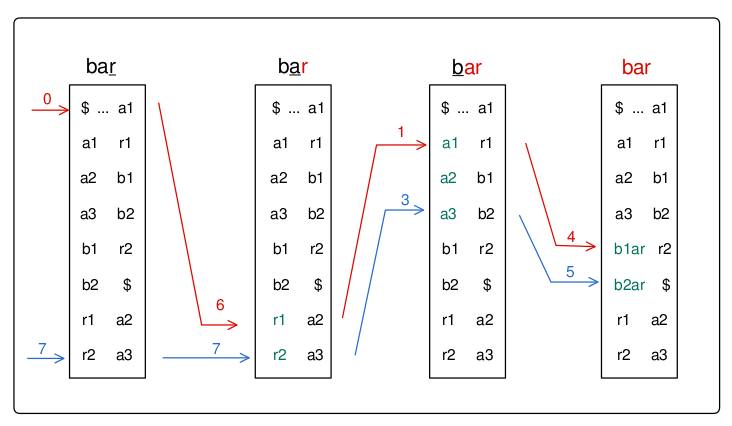
\includegraphics[width=12cm]{pictures/bar_1.png}
\caption{Backward search for pattern "bar" in string S using first and last column of BWT matrix. Updating indexes iteratively.}
\label{backwardSearch}
\end{figure}



\paragraph{Time Complexity}

The running time of the backward search on BWT depends on three factors; 
the length of the pattern P, the number of occurrence of P in the string and, 
more importantly, the access time of P in the suffix array.\\
The search algorithm consists of two phases, counting the number of occurrences of
a pattern and localization of their positions in the string.
The counting time is linear to the length of the P because at each iteration 
only one character of P is processed and length of the string doesn't have any 
impact on searching time which is one of the main reasons of using BWT for a large string like a genome.
On the other hand, the localization time is more affected by the number of occurrences 
of the pattern  because, for each occurrence of P, a look up at SA is needed.
\\\\

After introducing BWT and its properties and emphasising on its important job in pattern searching, in the following section the usage of BWT in an indexing data structure called FM-Index will be discussed\cite{fmindex}. 




%%%%%%%%%%%%%%%%%%%%%%%%%%%%%%%%%%%%%%%%%%%%%%%%%%%%%
\subsubsection{FM-Index (Full-text index)}

Paolo Ferragina and Giovanni Manzini in 2000, six years after BWT was 
published invented a self-index data structure that combines BWT with some 
small auxiliary data structures. It allows to efficiently search for the 
occurrences of an arbitrary pattern P as a substring of the string S as well 
as locate the position of each occurrence. They named it FM-Index for Full-
Text Index in minute space where minute space emphasises on memory efficiency.
The FM-Index is consist of two parts. The first part keeps the number of
occurrence of a pattern in string S using the LF-mapping property of the BWT (Sum table \emph{C}). 
And the second part stores the location of patterns in S ( in our case we used a Suffix Array)\cite{Wavthesis}.\\

\textbf{Sum Table}  The sum table must be stored completely because the frequency of characters
are independent of each other and can cause memory consumption problem \cite{Wavthesis}.
But in  fact, the number of alphabets in a string are usually very small in comparison to
the length of the string, especially in the case of a genome which is an alphabet size of 
four or five in contrast to a length of millions.
\\

\textbf{Occurance Table} The crucial part of FM-Index that needs to be 
both time and memory efficient is occurrence data structure\cite{Wavthesis}.
There are different implementations of occurrence data structure all aim toward making it faster and more memory efficient.
\\

\textbf{Partial Suffix Array} A suffix array is needed to determine the exact position of each pattern in the string S.
But saving the whole SA is very memory consuming , therefore,
it is more efficient to just save part of SA and recover the rest
of it recursively to reach the saved positions at any time it is necessary \cite{Wavthesis}.\\


%%%%%%%%%%%%%%%%%%%%%%%%%%%%%%%%%%%%%%%%%%%%%%%%%%%%%%

\subsubsection{A Wavelet Tree based FM-Index}

%A Wavelet Tree based FM-Index is used to create a simple and robust index structure for a genome with efficient time complexity on pattern searching.\\
We used a Wavelet Tree based FM-Index to create a simple and robust index structure for 
a genome with efficient time complexity on pattern matching.\\
\paragraph{Wavelet Tree}

A Wavelet Tree is a balanced binary tree to store strings as bit vectors in a 
compressed space\cite{navarroWavelet}\cite{Wavthesis}\cite{AlexBowe}.\\\\
Let s[0,n] be a binary sequence s[0,n] and $b \in {0,1}$ a finite alphabet. 
let $ rank_{b}(S, i)$ be the count of binaries b up to position i in string S 
and $ select_{c}(S,i)$  the position of $j_{th}$ occurrence of c in S.\\
The Wavelet tree is constructed recursively as follow:
\begin{enumerate}
    \item
		Take the string's alphabets and encode the first half of the alphabets as 0, and the second half as 1\cite {AlexBowe}:
    		$$\Sigma = \{ \$, a, b, r \}$$
			$$enc(\Sigma) = \{ 0, 0, 1, 1 \}$$
    \item
		Group each 0-encoded symbol, $\{ \$, a \}$, as a sub-tree;
    \item
		Group each 1-encoded symbol, $\{ b , r\}$, as a sub-tree;
    \item
		Repeat the procedure for each sub-tree until only one symbol has left.
\end{enumerate}
Wavelet tree for the string "Rhabarberbarbara" would look like this:
\begin{figure}[H]
\centering
\includegraphics[width=9cm]{pictures/wavelet.png}
%\includegraphics[width=0.75\textwidth, inner]{wavelet.png}
\caption{Wavelet tree for string "Rhabarberbarbara"}
\label{fig:barbWavlet}
\end{figure}

Construct the left subtree by taking all the 0-encoded symbols {\$,R,a,b} and
then divide them to new subtrees by re-encoding alphabet{0,0,1,1}.
Notice on the first level an "a" is encoded as a 0, but it is encoded as a 
1 on the second level and it becomes a 0 again at the leaf node.\\\\
The time complexity of Wavelet Tree to look for number of occurrences of a 
character up to specific position(OCC query) is $O(\log{}\mid\sum\mid)$.

%%%%%%%%%%%%%%%%%%%%%%%%%%%%%%%%%%%%%%%%%%%%%%%%%%%%%%%%%%%%%%%%%%%%

\section{Method}


\subsection{Benchmark design}

The features being covered by my benchmarking suite will be present in this section in addition to R-Candy's indexing structure and mapping algorithm.
\\\\
The evaluation is organized as follows: 
\\\\
\textbf{Mapping options}


\begin{itemize}

 \item \emph{Mapping quality threshold:} R-Candy uses the quality threshold (alignment score) to determine the accuracy of each alignment. 
 It is the probability of observing a read sequence given the alignment location. 

\end{itemize}
\textbf{Input properties}

\begin{itemize}

 \item \emph{Read length:}
The read length for ancient data varies between 25bps to 50bps and It's essential that its impact be considered for throughput evaluation.


 \item \emph{Genome type:} 
The human genome is used to test the performance of many aligners.
By the fact that each genome has different properties such as the different percentage of repetitive elements.
Thus, more than one genome should be used to reveal the effect of these properties. Two genomes are used in our evaluation, the human genome (version hg19) and a simulated genome based on the human genome.

\end{itemize}
\textbf{Scalability}
\\
The scalability of aligners could be considered in the aspect of parallel settings.
Some aligners support multithreading feature to increase their speed by allowing to use more than one CPU core.
The current version of R-Candy does not support multithreading while BWA does support multithreading.
 \\\\
\textbf{Accuracy evaluation}
\\
Each aligner is expected to align a set of reads while sometimes it does not happen due to its mapping algorithm or limitations in their default alignment parameters. Besides, some reads get align while violating the mapping principles of an aligner.
\\\\
\textbf{Usecase:}
\\
For example calculating Hamming distance between modern human genome and Neandertal genome .  
Calculating Hamming distance between two strings is the process of detecting the number of positions where the corresponding characters are different. In other words, it highlights the similarities and differences and helps us to learn about evolution. The alignment is the first step in this process which is very important to be done accurately.

%%%%%%%%%%%%%%%%%%%%%%%%%%%%%%%%%%%%%%%%%%%%%%%%%%%%%%%%%%%%%%%%%%%%%%%%%%%%%%%5
\subsection{Index Data Structure}

There are some challenges on the mapping of short reads\\
The first challenge is time and memory consumption: aligning billions of short
reads to an enormous genome (human genome of size about 3,200 Mbps), 
calls for an efficient algorithm with optimal query time and memory space.\\
Therefore, R-Candy builds a robust index structure with 
the efficient time complexity for pattern matching in a long sequence of a genome
called a Wavelet Tree based FM-Index that lessens its time complexity and memory footprint for mapping . 
\\\\
An overview of R-Candy's data structure is presented in Figure \ref{DSOverview}\cite{Wavthesis}.\\

\begin{figure}[H]
\centering
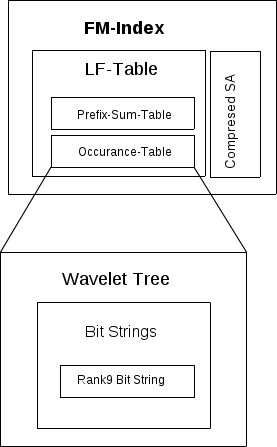
\includegraphics[width=4.75cm]{pictures/DSOverview2.png}
\caption{Overview of R-Candy's data structure }
\label{DSOverview}
\end{figure}


\subsubsection{Compressed Suffix Array}
The suffix array is needed to recover the position of patterns in the string
but storing the whole array is memory consuming, therefore, we used a
compressed version of SA to store some entries of SA.
The non-stored entries get retrieved by using LF-mapping.

\subsubsection{Prefix-Sum Table}
Prefix-Sum Table is a data structure used in FM-Index to store for every character c in string S the number of characters alphabetically smaller than c.

For the small alphabets of a genome, Prefix-Sum Table is stored
as a small array of alphabet size.

\subsubsection{Wavelet Tree}
A Wavelet Tree data structure encodes a character string to a
binary tree recall Section 2.4.4.1.\\

Construction of a Wavelet-Tree for $ S_{BWT} $ of string 'barbara':

%Therefore for implementation we just need the information of count table 
%\emph{C} and \emph{OCC} function.\\ 
%Now, we need a fast way of counting a given character in a prefix of our string.
%The first thing is to shrink it to bit vector using a Wavelet tree. 
 
\begin{table}[h]
\centering
  \begin{tabular}{ c c c c c c c c}
%  \begin{tabular}{| m{23pt} | m{23pt}| m{23pt}|}
   a  & r & b & b & r & \$ & a & a \\ 
  \hline
   0 &	1 &	1 & 1 & 1 & 0 & 0 & 0\\  
  \hline
%  0 & 1  & 2 & 3 & 4 & 5 & 6 & 7   
  \end{tabular}
\caption{The Wavelet tree binary encoded root node for "barbara" BWT.}
\label{wavlet-binary-barbara}
\end{table}


\begin{figure}[H]
\centering
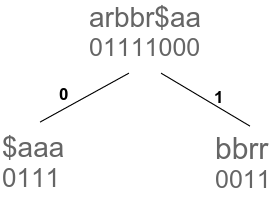
\includegraphics[width=4.75cm]{pictures/WavletBarbara.png}
\caption{Wavelet tree for "Rhabarberbarbara" string }
\label{Wavlet-barbara}
\end{figure}


A rank query can be done on  $O(\log{}\mid\sum\mid)$ time as is described below.
%After constructing the Wavelet tree (find at Figure 12), an rank query can be done on it. 

In order to calculate \emph{rank(5, a)} we use the following procedure
as illustrated in \ref{rank1}.\\
We know that \emph{enc(a)=1} at the root level by constructing wavelet
tree for the alphabet of  "Rhabarberbarbara" string.

\begin{enumerate}

    \item
		 Count the number of 1s in the range[1..7], at the root node, 
		 given by \emph{rank(7,0)=5 }. This is the index to query in 0-child.
		 
    \item
		As 'a' is encoded as 1 at this child, calculate \emph{rank(5,1)=4}. 
		We use 4 as an index for next branch.

    \item
		\emph{rank(4,0)=2} as 'a' is encoded as 0 here and return 2 as our
		 result since we are at the leaf node.

\end{enumerate}

\begin{figure}[H]
\centering
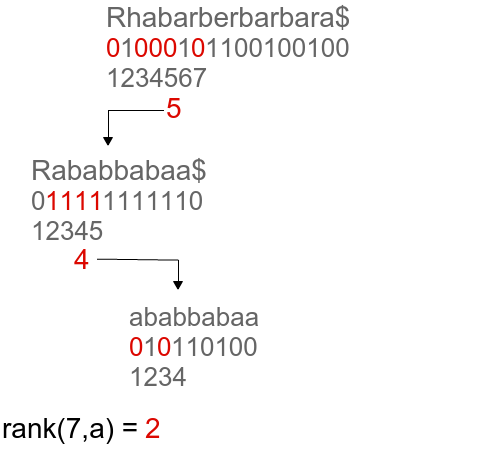
\includegraphics[width=7cm]{pictures/rank1.png}
\caption{The rank(7,a) over Wavelet tree for "Rhabarberbarbara" string }
\label{rank1}
\end{figure}

The space usage is given by this structure.
Bits proportional to the depth of  Wavelet tree are needed to encode
each character giving memory usage proportional to $H_{0}$(empirical entropy)\cite{entropy}.\\

We define \emph{$rank(n,0)= n- rank(n,1)$} and implement \emph{$rank(. , 1)$}
using the Rank9 structure described below.


\subsubsection{The rank9 Data Structure}

%In this part, the layout of our data structure will be introduced.\\	

The rank9 data structure was first proposed by Vigna, Sebastiano \cite{rank9}.
The main idea is to turn a bit sequence into a bit string that supports
rank queries in $O(1)$ time.\\

Consider an array of 64-bit words represented as bit array \emph{b}.
The bit at position p is stored in bit (\emph{p} mod 64) of
$ [p \backslash 64]$ \cite{rank9}.\\ 
Let a \emph{basic block} be a subsequence of eight words 
starting at bit position \emph{p}.\\
To construct the rank9  we divide the bit string into several basic
blocks and then divide these blocks further, into words of 64 bits.\\
We store the 512 bits in a \emph{basic block} and two words (as described in \cite{rank9}):

\begin{enumerate}

	\item The first word (first-level count) contains the total number of
	 1s till that position \emph{(rank(p)});
	
	\item The second one contains the seven 9-bit values (second-level counts)
	 \emph{rank(p + 64k)- rank(p)} , for 1 $\leq$ k $\leq$ 7,each shifted left by \emph{9(k-1)} bits.
	
\end{enumerate}

To construct the rank9  we divide the bit string into several basic blocks.
For each basic block boundary, a sum of previous ranks (first-level rank) and the address of  
stored offset values(second-level rank) are stored which gives us an efficient rank query time. \\

%And when we want to rank a position \emph{p}, use following formula:\\

%To construct the rank9 layout, we divide the bit vector of Wavelet tree into several blocks and then divide these blocks further, into words of 64 bits.

For each block, we store:\\\\
\centerline{$ block[i].total= rank(i*512)$}\\\\
\centerline{$ block[i].subtotal[j]= rank(i*512 + (j+1)*64)-block[i].total$}\\\\
\centerline{$ b[i*8]=raw[i*512..i*512+(k+1)*64)] $}\\\\
\centerline{$ OCC_{1}(x)=block[i].total+block[i].subtotal[j-1]+popcount(b[i*8 + j],0,k)$}



\[ where
\begin{cases}
	i=[ x \backslash 512 ]\\
	j=[(x \% 512 )\backslash 64 ]\\
	k=[ x \% 64  ]\\
\end{cases}
\]

%%%%%%%%%%%%%%%%%%%%%%%%%%%%%%%%%%%%%%%%%%%%%%%%%%%%%%%%

\subsection{Alignment}

Semi-global \footnote{Reads are globally aligned(fully aligned)where the reference is
locally aligned (with some gaps at the end of the reference string)} alignment results
have been produced by R-Candy as a result of mapping sets of short strings against 
long reference (for instance, strings of length $\geq 25$ bps aligned to a refernce of length 3.2 Gbs).
To calculate the highest similarity score(lowest Levenshtein distance) between two strings, 
we fill out the desirable and reference in the Y-axis and X-axis respectively.
Starting from the top left with score zero the score matrix leads us to the 
maximum score in the bottom right position.

Comparing every individual string with a corresponding-length reference is not feasible in
terms of memory consumption(exponential to the number of insertion and deletion allowance) 
therefore alternative heuristic which takes the following characteristics into account is needed: 


\begin{itemize}

\item Dealing with ancient DNA, we have very short reads and we do not allow for more than one INDEL, which reduces the memory usage.\\

\item 
In our case, the reference is a tree, not a sequence as our genome sequence is converted to 
a Wavelet Tree data structure.
We simply say that we split the reference into branches for reference. So we have a reference that gives for 
any tree the outgoing edges from the root which all have letters  as a label and then an attached tree.
We will be able to start from the beginning (tree's root) and look for the query in branches which uses the Depth First Search(DFS) algorithm. 
It also is cheaper in terms of memory because using a tree as a reference makes it reusable.
All needs to be done is to backtrack one step and look at another branch, so most of the matrix is reused.\\


%\item When we are done with query doesn't matter its reference left over. 
%We always start from the root node but we don't end up at the leaf,
%we end up anywhere when we are done with the query. In fact, 
%run down all the queries that are as long as your query.\\

\item
As we always start from the root note:
\begin{enumerate}
 \item When we are done with the query it does not matter if its corresponding reference if not finished yet.
 
 \item Not to end up at the leaf while the query has not finished yet,
we run down all the queries that are as long as our query.

\end{enumerate}
%\item We also introduce a bound 'b' which is the maximum score that we are willing to endure.
%We put some limit on the computed score of each cell
%and if we never find anything  below that limit, we say we did not find an alignment but as 
%soon as finding an alignment, you lower the limit because you want a better one calling it Branch and Bound\cite{}.\\\\

 \item Following the Branch and Bound heuristic, we increase the lower bound of the introduced score that we are willing to endure. In the case of not finding anything below that limit, no alignment found gets report.
 
\end{itemize}
Given a non-empty sequence $q\in (q_{1}..q_{n})$, we want to align it to 
another non-empty sequence (reference)$r\in (r_{1}..r_{n})$:\\\\



\begin{figure}[H]
\centering
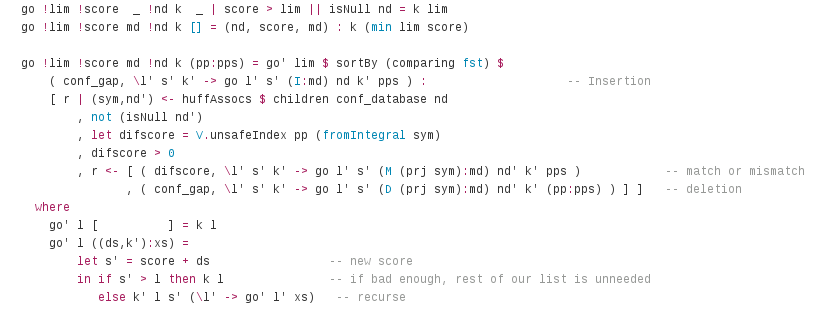
\includegraphics[width=15cm]{pictures/A_HS.png}
%\caption{ROC curve for simulated reads with deamination damage aligned to the simulated genome
 %        with deamination parameters.}
\label{formula}
\end{figure}


We take the minimal score of three options match/mismatch, insertion and 
deletions, as described in the above code.
The score that we have so far plus match score between q and r and pair it 
with Match operation (M) in the CIGAR field \cite{samtools}.\\
In the case of insertion (I) in the MD field \cite{samtools}: 
calculated score so far plus insertion score(penalty) pair with insertion
operation and CIGAR field for insertion.
The same procedure applied to deletion operation.

 
\subsubsection{Scoring}
Let $\sigma$ and $\delta$ be the single stranded and the double stranded
deamination rates.  Let $l$ be the length of the read being aligned.  

For double stranded library preparation, let $\lambda$ be overhang
length parameter.  For every position $i \in [0..l-1]$ define

\begin{align*}
p_{fwd} &= \lambda^{i+1} \\
p_{rev} &= \lambda^{l-i} 
\end{align*}

For single stranded library preparation, let $\lambda_s$, $\kappa_s$ be
the 5' overhang length parameter and the 3' overhang parameter.  Let $l$
be the length of the read being aligned.  For every position $i \in
[0..l-1]$ define

\begin{align*}
p_{fwd} &= \lambda_s^{i+1} + \kappa_s^{l-i} - \lambda_s^{i+1} \kappa_s^{l-i} \\
p_{rev} &= 0
\end{align*}

Now define effective substitution probabilities

\begin{equation*}
p_{C} = \sigma p_{fwd} + \delta (1 - p_{fwd}), \quad
p_{G} = \sigma p_{rev} + \delta (1 - p_{rev}) 
\end{equation*}

Scoring a base at position $i$ with quality score $q$ involves
deamination, divergence and error.  We assume both a trivial error model
and a trivial model of evolution, where all possible changes occur with
a uniform rate derived from the quality score and a uniform rate given
by parameter $D$, respectively.  Define 

\begin{equation*}
\epsilon_0 = {10^{-q/10}}/4, \quad \epsilon = \epsilon_0 + D/3 - \epsilon_0 D/3
\end{equation*}

and the complete substitution matrix becomes (reference base in columns,
query base in rows, both in the order A, C, G, T):

\begin{equation*}
\left( \begin{array}{cccc}
1 - 3 \epsilon &       \epsilon                            &       \epsilon + p_{G} - 4 \epsilon p_{G} &       \epsilon \\
      \epsilon & 1 - 3 \epsilon - p_{C} + 4 \epsilon p_{C} &       \epsilon                            &       \epsilon \\
      \epsilon &       \epsilon                            & 1 - 3 \epsilon - p_{G} + 4 \epsilon p_{G} &       \epsilon \\
      \epsilon &       \epsilon + p_{C} - 4 \epsilon p_{C} &       \epsilon                            & 1 - 3 \epsilon 
\end{array} \right)
\end{equation*}

Alignment scores are simply the sum of the natural logarithms of the
entries in that matrix for every aligned base, plus a penalty for
insertions and deletions.  We use linear gap costs with a cost of $G$
per inserted or deleted base, where $G$ is a free parameter again.



%%%%%%%%%%%%%%%%%%%%%%%%%%%%%%%%%%%%%%%%%%%%%%%%%%%%%%%%
\section{Test Data}

%In the past few years, the development of new DNA sequencing technologies made it possible to get DNA from ancient organisms.
%The analysis of such a data regularly by aligning it to the genome of closely related modern species is a big challenge in human evolution studies.
A number of alignment software are developed to map such a dataset where 
simulated data is essential to guide the new software development and 
evaluating their performance.

Therefore, simulating data that captures the most crucial characteristics 
of real data is the key point in evaluation of the new software.\\

To satisfy this, I developed a genome and NGS read simulation program to evaluate 
the performance of R-Candy in different cases.

%%%%%%%%%%%%%%%%%%%%%%%%%%%%%%%%%%%%%%%%%%%%%%%%%%%%%%%%%%%%%%%%%%%%%%%%%%
\subsection{Genome Simulation}

Generally, every genome consists of some repeated stretch of sequences which make 
the alignment of short reads from these repetitive parts very difficult due to 
finding the true alignment between the same repeated sequences.

In order to make the software evaluation more informative, we decided to first 
test the aligner with a simulated genome that has no short repeated sequences 
and check its accuracy and performance where we know the true alignment of each 
read.

In this thesis I used a probabilistic model called \emph{Markov Chain} model 
\footnote{More specifically \nth{1} Order Markov Chain as my future state only 
depends on my current state} to simulate a genome by generating stretch of 
nucleotides (A, C, G, T bases) in a way that  keeps the base composition of the 
real reference genome but not generates repeats.


\subsubsection{\nth{1} Order Markov Chain}
A Markov chain graphically can be drawn as a collection of states, 
each corresponds to a particular nucleotide (A, C, G, T) with arrows
between them like the following (Figure \ref{MC}). 
%The conversion probability of each state to the other state is 
%associated with each arrow in the graph. 
\\\\ 
Having a set of states,  $ S= \{ A, C,  G, T \}$  and probability
parameter  associated with arrows in the figure which determines the
probability of transferring from one state to the next state (Transition)
or staying on the same state (Emission).

\begin{figure}
 \begin{center}
  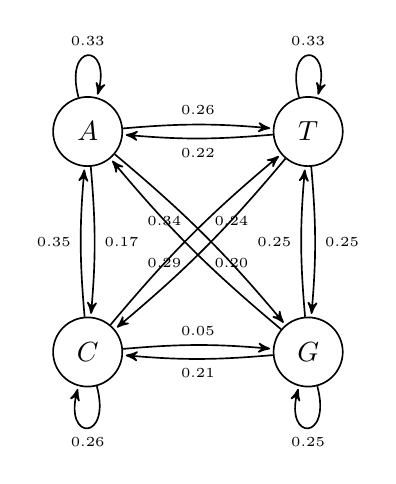
\begin{tikzpicture}[->,>=stealth',shorten >=1pt,auto,node distance=2.8cm,
                    semithick,bend angle=5]
   \tikzstyle{every state}=[fill=white,draw=black,text=black]

   \node[state]         (A)              {$A$};
   \node[state]         (T) [right of=A] {$T$};
   \node[state]         (C) [below of=A] {$C$};
   \node[state]         (G) [below of=T] {$G$};
  
   \path (A) edge [bend left]  node {\tiny 0.26} (T)
  			edge [loop above] node {\tiny 0.33} (A)
            edge [bend left]  node {\tiny 0.17} (C)
            edge [bend left]  node {\tiny 0.24} (G)
        (T) edge [loop above] node {\tiny 0.33} (T)
            edge [bend left]  node {\tiny 0.22} (A)
            edge [bend left]  node {\tiny 0.20} (C)
            edge [bend left]  node {\tiny 0.25} (G)
        (C) edge [bend left]  node {\tiny 0.34} (T)
            edge [loop below] node {\tiny 0.26} (C)
            edge [bend left]  node {\tiny 0.05} (G)
            edge [bend left]  node {\tiny 0.35} (A)
        (G) edge [loop below] node {\tiny 0.25} (G)
       	    edge [bend left]  node {\tiny 0.21} (C)
        	edge [bend left]  node {\tiny 0.29} (A)
            edge [bend left]  node {\tiny 0.25} (T);
  \end{tikzpicture}
  \caption{Trained \nth{1} order markov chain based on human reference genome}
  \label{MC}
 \end{center}
\end{figure}


%\begin{center}[H]
% \begin{tikzpicture}[->,>=stealth',shorten >=1pt,auto,node distance=3cm,
%                    semithick, bend angle=5]
%  \tikzstyle{every state}=[fill=white,draw=black,text=black]

%  \node[state]         (A)              {$A$};
%  \node[state]         (T) [right of=A] {$T$};
%  \node[state]         (C) [below of=A] {$C$};
%  \node[state]         (G) [below of=T] {$G$};
  
%  \path (A) edge [bend left]   node {\footnotesize 0.3} (T)
%  			edge [loop above]  node {\footnotesize 0.3} (A)
%            edge [bend left] node {\footnotesize 0.2} (C)
%            edge [bend left=5] node {\footnotesize 0.2} (G)
%        (T) edge [loop above] node {\footnotesize 0.3} (T)
%            edge [bend left]  node {\footnotesize 0.2} (A)
%            edge [bend left=5]  node {\footnotesize 0.2} (C)
%            edge [bend left]  node {\footnotesize 0.3} (G)
%        (C) edge [bend left=5]  node {\footnotesize 0.3} (T)
%            edge [loop below] node {\footnotesize 0.3} (C)
%            edge [bend left]  node {\footnotesize 0.1} (G)
%            edge [bend left]  node {\footnotesize 0.3} (A)
%        (G) edge [loop below] node {\footnotesize 0.3} (G)
%        	edge [bend left]  node {\footnotesize 0.2} (C)
%        	edge [bend left=5]  node {\footnotesize 0.3} (A)
%            edge [bend left]  node {\footnotesize 0.2} (T);
% \end{tikzpicture}
%\end{center}



As mentioned above these probabilities are called \emph{transition or emission 
probabilities}, which are calculated by counting the number of state given its 
previous state ($ A \rightarrow A, A\rightarrow C, A \rightarrow T, A \rightarrow 
G, C \rightarrow C,$ ...) in the genome of interest; see the Table \ref{transition-table}
(Filled with human reference genome bases consistency).And then create a 
\emph{Transition Matrix} by calculating the frequency of seeing each transition,
as shown in Figure \ref{transition-matrix}.\\

\begin{table}[h]
  \begin{tabular}{ |  p{1cm} | p{2cm} | p{2cm} | p{2cm} | p{2cm} |}
    \hline
  	%\textbf{Type} & \textbf{Read length } &\textbf{Running time(s) } 
  	%&\textbf{Speed \hspace{35pt}(no. of reads/s)} \\ \hline
  	  
 	             & A   & C & G & T \\ \hline
      A  & 279630175  & 143865843 & 199830254 & 220834783 \\ \hline
 	  C	 & 207298683  & 148996334 & 28155478 & 199938031\\ \hline
 	  G	 & 169559114  & 121898050 & 149073778 & 144192413\\ \hline
 	  T  & 187672847  & 169629108  & 207663790 & 280419080\\ \hline
      
 	  
   \end{tabular}
%\caption{Transition number for a genome sequence of length 
%1G bp and chromosomes of length 250M bp.}
  \caption{Transition number for human reference genome}
 \label{transition-table}
\end{table}

%And then calculate the frequency of seeing each transition 
%called \emph{Transition Matrix}, as shown below.


\begin{figure}[H]
 \centering
\[
T = 
 \begin{pmatrix}
   &  A  & C & G & T  \\
 A & 0.331252 & 0.170425 & 0.236721 & 0.261603  \\
 C & 0.354727 & 0.254961 & 0.0481794 & 0.342132  \\
 G & 0.289982 & 0.208471 & 0.254948 & 0.246599  \\
 T & 0.221997 & 0.200653 & 0.245644 & 0.331706 \\
  
 \end{pmatrix}
\]
 \caption{Transition Matrix for human reference genome}
 \label{transition-matrix}
\end{figure}

Besides specifying the transition probabilities, the probability of starting 
state( state \emph{S} in the graph) is required. In our case as we don't have
special interest on starting from particular state all four state are equally 
probable to get started. And no specific probability for an end state defined as 
E because the sequence can end anywhere (Figure \ref{MC_SE}).


\begin{figure}
 \begin{center}
 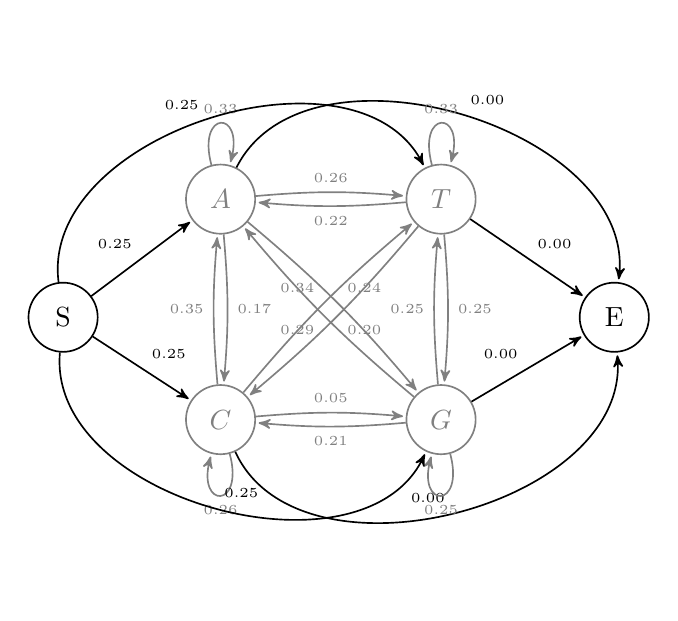
\begin{tikzpicture}[->,>=stealth',shorten >=1pt,auto,node distance=2.8cm,
                    semithick,bend angle=5]
  \tikzstyle{every state}=[fill=white,draw=gray,text=gray]

  \node[state]         (A)              {$A$};
  \node[state]         (T) [right of=A] {$T$};
  \node[state]         (C) [below of=A] {$C$};
  \node[state]         (G) [below of=T] {$G$};
  \node[state]         (S) [draw=black, text= black]at (-2,-1.5) {S};
  \node[state]         (E) [draw=black, text = black]at (5 ,-1.5) {E};
  
  \path (A) edge [gray, bend left]  node {\tiny 0.26} (T)
  			edge [gray, loop above] node {\tiny 0.33} (A)
            edge [gray, bend left]  node {\tiny 0.17} (C)
            edge [gray, bend left]  node {\tiny 0.24} (G)
            edge [bend left=80]  node {\tiny 0.00} (E)
        (T) edge [gray, loop above] node {\tiny 0.33} (T)
            edge [gray, bend left]  node {\tiny 0.22} (A)
            edge [gray, bend left]  node {\tiny 0.20} (C)
            edge [gray, bend left]  node {\tiny 0.25} (G)
            edge   			  node {\tiny 0.00} (E)
        (C) edge [gray, bend left]  node {\tiny 0.34} (T)
            edge [gray, loop below] node {\tiny 0.26} (C)
            edge [gray, bend left]  node {\tiny 0.05} (G)
            edge [gray, bend left]  node {\tiny 0.35} (A)
            edge [bend right=80]  node {\tiny 0.00} (E)
        (G) edge [gray, loop below] node {\tiny 0.25} (G)
       	    edge [gray, bend left]  node {\tiny 0.21} (C)
        	edge [gray, bend left]  node {\tiny 0.29} (A)
            edge [gray, bend left]  node {\tiny 0.25} (T)
            edge   			  node {\tiny 0.00} (E)
        (S) edge   			  node {\tiny 0.25} (A)
       	    edge   			  node {\tiny 0.25} (C)
        	edge [bend right=80]  node {\tiny 0.25} (G)
            edge [bend left=80]  node {\tiny 0.25} (T)
       
            ;
;
 \end{tikzpicture}
 \caption{Trained \nth{1} Order Markov-Chain based on human reference genome with start and end state}
 \label{MC_SE}
 \end{center}
\end{figure}


The simulation program asks for the length of the genome and then the Markov chain 
model starts randomly from one of the states and continuously walk between states 
based on their probabilities on transition matrix till the number of visited stateds 
is reached the given genome length which could equally be at any state. \\\\

%%%%%%%%%%%%%%%%%%%%%%%%%%%%%%%%%%%%%%%%%%%%%%%%%%%%%%%%%%%%%%%%%%%%%
\subsection{Read Simulation}

The second part of my test data preparation is about simulating ancient DNA reads 
sequenced by Illumina machine.

Read has been sequenced with \emph{post-mortem }damage \cite{damagepattern} (the 
specific characteristics of ancient DNA), and sequencing errors \cite{phred1} (from
Illumina platform) plus additionally substitution for divergence/mutation.


%%%%%%%%%%%%%%%%%%%%%%%%%%%%%%%%%%%%%%%%%%%%%%%%%%%%%%%%%%%%%%%%%%%
\subsubsection{Divergence}

By definition \quotes{ divergence is the separation
of a population's gene pool from the gene pools of other populations 
due to mutation, genetic drift, and selection \cite{divergence2}.}\\

Introducing divergence property which also is used in R-Candy's mapping strategy to my simulation is next step in my simulation process. 

To understand how much divergence impedes mapping, 
I simulated reads with a small number (0..6) of differences to the reference genome.
And ran R-Candy with a default value for different datasets of reads with a different number of divergence substitution rates to evaluate the accurate of its alignment while aligning reads to close or far genomes.

%%%%%%%%%%%%%%%%%%%%%%%%%%%%%%%%%%%%%%%%%%%%%%%%%%%%%%%%%%%%%%%%
\subsubsection{Deamination}

A high nucleotide misincorporation rate of  deamination of cytosine(C) to uracil, code as thymine(T) are the unique characteristics of ancient DNA as the result of \emph{post-mortem} DNA damage\cite{mapdamage2}\cite{damagepattern}.\\ 

Observation in the recently introduced single-stranded library preparation protocol
has shown a significant increase in C to T substitution rates at the read terminals\cite{mapdamage2}.\\

A model developed by Philip Jonson \cite{mapdamage2} is used
to simulate \emph{post-mortem} deamination as the followings:

For single stranded library preparation,
let $\sigma$ and $\sigma\prime $ be deamination rate in the 5' and 3' overhangs respectively and $\lambda$ be overhang length parameter. 

Let  $\delta$ and $l$ be the
deamination rate at the middle(non-overhang) parts and the length of the read being aligned.\\

The DNA damage transition matrix is defined as:

$$ P_{dam} = 
 \begin{pmatrix}
  1 & 0 & 0 & 0 \\
  0 & 1-p_{ct} & 0 & p_{ct} \\
  0  & 0  & 1 & 0  \\
  0 & 0 & 0 & 1 
 \end{pmatrix}$$
 

The probability of damage for each base is defined  
as\cite{mapdamage2}:\\
%Where the base-specific damage probabilities are defined as\cite{mapdamage2}:\\
$$ p_{ct}(\sigma, \delta, \lambda, i) = ( \lambda_{i} \sigma + \delta(1 - \lambda_{i})) $$
 
It uses a geometric distribution to calculate the length of the overhang at both ends of a sequence based on certain deamination parameters.
 

The probability of being in overhang is provided by the user as the success fraction in the geometric cumulative distribution function (CDF).


We assume the probability of each base being in overhang is independent than the other bases.\\

$$Pr( X=k ) = 1 - (1 - p)^{k}$$
$$ k = 1, 2, 3, ... $$


The simulation program first calculates the overhang length given the user-specified success fraction value.


And then uses the user-specified substitution ratio numbers,
 $ \sigma $ and $\sigma\prime $, for substitution of 
 the $ C \rightarrow T $ 
in overhangs which usually is higher than the deamination substitution ratio, $delta$, in non-overhang parts of aDNA reads.

 
%%%%%%%%%%%%%%%%%%%%%%%%%%%%%%%%%%%%%%%%%%%%%%%%%%%%%%%%%%%%%%%%%%%%%%%%%%%%%%%%%%%%%%%%%%%%%% 
\subsubsection{Sequencing Error}
 

A sequencing error is an incorrect identification of a nucleotide base resulting to an inaccurate read. 
due to the error in the base calling of the sequencing machines, there is no precise DNA sequencing. \\
A quality score indicating the confidence of correctly seeing a base is assigned to each base of a read sequence.\\
Different sequencing methods have different quality score leading to variable sequencing error. These errors become visible when aligning a read to a reference string.\\
The main sequencing error for Illumina platform is base substitution due to reading out one base at a time \cite{art}.\\

The substitution error probability is calculated by the base quality score along with the called base.\\


The output data of sequencing machines significantly differs in quality for several reasons ( for illustration, see Ewing et al. 1998) therefore, an effective measure for the reliability of such a data is vital \cite{phred1}.\\

In order to assess the accuracy of sequencing data, base calling accuracy by Phred quality score (Q score) is the most widely used metric. It demonstrates the probability of an error in base calling by a sequencer.\\

Phred quality scores are defined as \cite{phred2}:

$$ Q = -10  log_{10}P   $$
$$  or $$
$$ P = 10 ^ { \frac{-Q}{ 10 } } $$

For instance, if Phred score of a base is Q40, it means the probability of an incorrect base call is a 1 in 10000 which shows 99.99\% base call accuracy \cite{IlluminaPhred}. \\  

In order to implement sequencing error for simulated reads, There are two
options in my program (readSim):

The first option uses a next-generation sequencing read simulation software, (ART).
ART generates sequencing reads based on different sequencing technology platforms
(454, Illumina, SOLiD) criteria[35].

ART simulates the substitution error probability, base on the base
quality score distribution reported by large training datasets[35].

In order to use ART in readSim you just need to specify the sequencing platform 
and the length for generating base quality scores. Despite the user-friendly 
and easy working features of ART, it has a low quality score rate compared
to the empirical data\cite{bwa} which leads to the high sequencing error rate.

For this reason, there is a second option in readSim that simulates
sequencing error based on an empirical data.

The implementation looks at the qualities of the sequencing error profile assigned to it base by base and generates a 
distribution table for it. Then calculates probability mass function (PMF) 
which is the error quality frequencies at each cycle for both forward and 
reverse reads. At the next step, cumulative distribution function (CDF) is calculated 
by summing up the quality frequency of each base with all quality bases before it. 
Given the CDF distribution, the quality score of bases in a read determined using a 
random number to sample.




%%%%%%%%%%%%%%%%%%%%%%%%%%%%%%%%%%%%%%%%%%%%%%%%%%%%%%%
\subsection{Simulating Endogenous Sequences}

Ancient DNA extracts consist of a low amount of endogenous DNA which used to be a big problem at evolution researchers until the recent technology of sequencing polymerase chain reaction (PCR) \cite{PCR} made it possible to amplify DNA sequences and produce high coverage data for deeper studies on human origins.
\\\\
My endogenous read simulation process starts
\begin{itemize}
 \item First by uniformly sampling reads over the reference genome.

 \item Second, introducing a small number of differences to 
 reads in order to simulate different divergence rates.

 \item Third, simulating \emph{post-mortem} deamination damage based on deamination parameters (like, deamination rate in overhangs and non-overhang parts and probability for calculating the overhang lengths) by users. 

 \item Fourth,  adding the specific types of errors coming from sequencing machine to the reads.
\end{itemize}
%%%%%%%%%%%%%%%%%%%%%%%%%%%%%%%%%%%%%%%%%%%%%%%%%%%%%%%%%%
\subsection{Simulating Microbial Sequences}

   

Ancient DNA extracts are highly contaminated by mostly environmental microbes that always make the recognition of endogenous and exogenous DNA hard for aligners.
Although there is a database of known bacteria DNAs that could help us to detect bacterial sequences and don't mix them with endogenous 
DNA sequences but still there are a lot of unknown bacterial contamination.
\\\\
In order to have a realistic simulation of ancient DNA, we decided to simulate microbial DNA sequences besides our genomic DNA reads simulations.
\\\\
The microbial reads simulation process starts

\begin{itemize}

 \item First by generating a totally random string of DNA nucleotides (A, C, G, T) for a given length.

 \item Second, Add the \emph{post-mortem} deamination damage to 
the reads which is the substitution of C base by T based on deamination parameters to simulate the ancient microbial sequences.


 \item Third, introducing sequencing machines errors 
 to the read simulation.

\end{itemize}



%%%%%%%%%%%%%%%%%%%%%%%%%%%%%%%%%%%%%%%%%%%%%%%%%%%%%%%%%%%%%%%%
\section{Results and Discussion}

%%%%%%%%%%%%%%%%%%%%%%%%%%%%%%%%%%%%%%%%%%%%%%%%%%%
%\subsection{Implementation}

The R-Candy is an alignment program for 
short sequences (30-50 bps) of ancient DNA based on BWT of the reference genome written in Haskell. 
It performs semi-global alignment for single end reads, supports pair-end aligning, 
generates alignment score and produces multiple hits if required.

The R-Candy's output is a BAM file. It is the binary version of a SAM file in order to compress data reasonably well. 
A SAM file (Sam Alignment/Map format) is a tab-delimited text file that contains sequence alignment data.   
More information about these formats is available on the SAM Tools website: http://samtools.sourceforge.net.

%R-Candy's documentation and source code are freely available at (https://github.com/udo-stenzel/r-candy.git).

%My genome/read simulation software written in C++ is freely available at\\ 
%(https://github.com/Homa1127/simulateGenome.git).



%%%%%%%%%%%%%%%%%%%%%%%%%%%%%%%%%%%%%%%%%%%%%%%%%%%%%%%%%%
%\subsection{Evaluated Programs}

To evaluate the performance of R-Candy, we tested an additional Burrows-Wheeler 
transform-based alignment program: BWA \cite{bwa}
on the number of simulated datasets modeling different types of reads. \\
BWA is a widely used aligner for short reads, it indexes reads using Burrows-
Wheeler transform of the reference genome, and allows gaps and mismatches for alignments\\


%%%%%%%%%%%%%%%%%%%%%%%%%%%%%%%%%%%%%%%%%%%%%%%%%%%%%%%%%%%%%%%%
\subsection{Evaluation criteria}

The evaluation is done based on three aspects, namely, 
the mapping percentage, the throughput and memory footprint.

\begin{itemize}

 \item The mapping sensitivity or percentage:
the number of correctly mapped genomic reads divided by the total number of endogenous reads versus the number of aligned simulated microbial reads 
divided by the total number of simulated microbial reads.

 \item The aligner's throughput: the number of mapped reads per second(bps/sec).

 \item The memory footprint: the required memory by the tool for indexing reference string, process the reads and storing them. 

\end{itemize}


The mapping sensitivity is divided into two parts, correct(true positives) and incorrect (false positives) alignments.

There are different ways of calculating the incorrect alignments. For simulated reads,
the percentage of reads mapped to the incorrect location (aligned to a position differ than the original position in the genome where the read was originally extracted from) which is a common definition of error used in many studies \cite{ErrorDef}. 

But, this na\"{\i}ve definition of the correctness of an alignment has some problems. For example after applying sequencing error and deamination damage on the reads, the read does not exactly match the original genomic position. And it would be a problem when the aligner chooses the location for a read with no or fewer mismatches over the original location. In this case, the result will be poorly judged as an incorrect mapping despite the more accurate matching position has been chosen. 
The problem has been managed using mapping quality/alignment score information. Such that a correct alignment of a read is defined as being to its original genomic location and having the alignment score/mapping quality fewer/greater than a certain threshold. 



%%%%%%%%%%%%%%%%%%%%%%%%%%%%%%%%%%%%%%%%%%%%%%%%%%%%%%%%
\subsection{Specificity and Sensitivity}


The sensitivity reported is the number of correctly mapped simulated
endogenous reads divided by the total number of simulated endogenous reads.\\ 
The fall-out is the number of aligned simulated microbial reads 
divided by the total number of simulated microbial reads.


%%%%%%%%%%%%%%%%%%%%%%%%%%%%%%%%%%%%%%%%%%%%%%%%%%%%%%%%%%%

\subsection{Evaluation on Simulated Genome}

To simulate a genome we used human reference (as a training dataset) and first-order Markov chain as a training model. 

The reads are sampled from the simulated genome 
with additional properties in the case of different scenarios.

Knowing the true alignment of the reads, we evaluated the alignment accuracy.\\ 
%Generated data are in different lengths 25, 30, 35 and 40 with a set of errors, (divergence, deamination, and sequencing error). \\
%Knowing true coordinates of simulated read, I align them with two aligners (R-Candy and BWA) and evaluate their outputs.

%%%%%%%%%%%%%%%%%%%%%%%%%%%%%%%%%%%%%%%%%%%%%%%%%%%%%%%%%%%%%


\subsubsection{Evaluation Scenarios}


\emph{Post-mortem} damage (deamination) is a specific characteristic of ancient DNA that none of existing aligners for short
reads are taken into account except R-Candy.\\

To show the impact of deamination on alignment, I divided my evaluation into six parts:

\begin{enumerate}
 
 \item
 
  \begin{itemize}
   \item \textbf{Data:} simulated reads with deamination damage
with $ \sigma = 0.9$, $ \sigma\prime = 0.93 $, $\delta = 0.02 $,  and $\lambda = 0.3 $ parameters for Philip Johnson deamination model and extra substitutions due to different divergence rate(see Section 4.2.1) and sequencing error using empirical quality distribution data and also sequencing error provided by ART for Illumina platform.

  \item \textbf{Reference genome:}  align to a simulated genome based
 on the human genome.

  \item \textbf{Aligners:} R-Candy with damage parameters and alignments score 20. \\
BWA with default parameters (there are no damage parameters in BWA)
and its modified version for ancient data with the number of mismatches ( 0.01 ) and the number of gap opens ( 2 ).

  \end{itemize}

\begin{figure}[H]
\centering
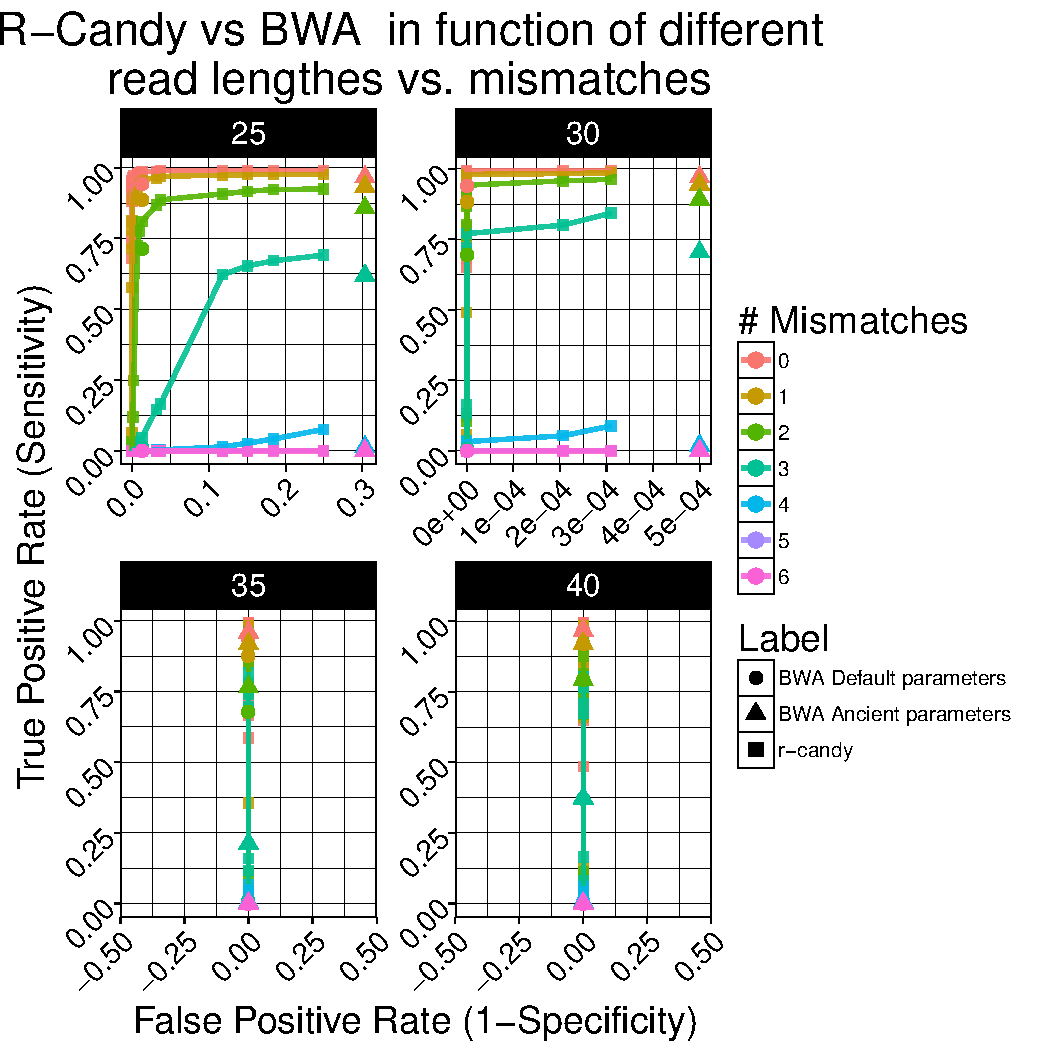
\includegraphics[width=12cm]{pictures/bROC_DS1_emp.pdf}
\caption{ROC curve for simulated reads with deamination damage and sequencing error by empirical quality distribution data, aligned to the simulated genome
         with true deamination parameters.}
\label{DS1_emp}
\end{figure}

\begin{figure}[H]
\centering
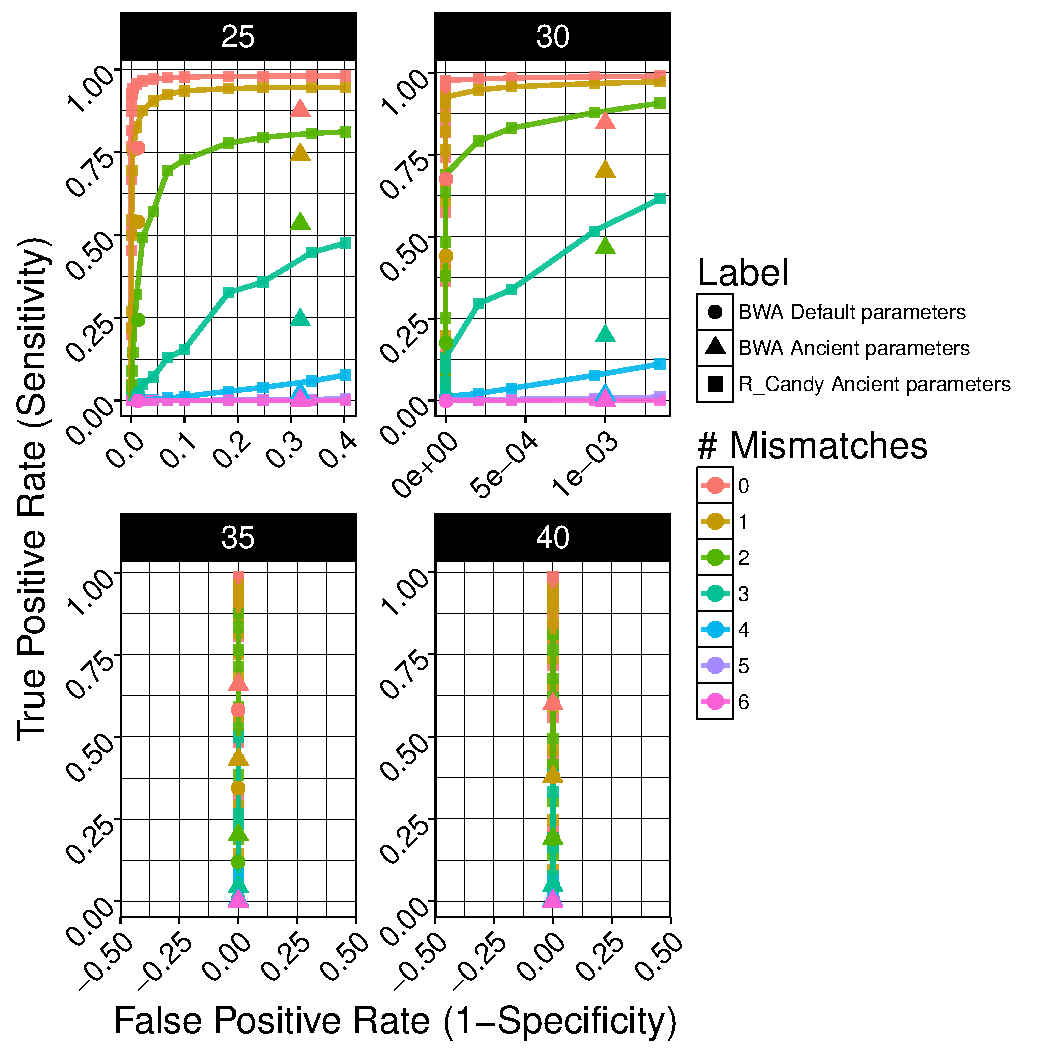
\includegraphics[width=12cm]{pictures/bROC_DS1_ART.pdf}
\caption{ROC curve for simulated reads with deamination damage and sequencing error by ART, aligned to the simulated genome
         with true deamination parameters.}
\label{DS1}
\end{figure}


The ROC curve plot shows R-Candy with different AS numbers.
And in the case of multiple best hits reported by R-Candy, just one hit has been chosen arbitrarily to do a fair comparison between R-Candy and BWA which reports one best hit per each read.
As the result shows, R-Candy archives the highest rate of sensitivity in all four lengths.

Length 25 is a very challenging length for aligners, where any small change in the read bases could make a perfect match in another part of the reference genome and recognizing the true genomic position very hard. 

In the case of deaminated reads with only sequencing error, no extra substitution (the plot with zero mismatches), the sensitivity rate for R-Candy is 99\% compare to BWA with ancient data parameters 97\% and BWA with default parameters 94\%. 
Introducing extra mismatches to the reads, we see sensitivity decreasing for both aligners as expected.

As is expected, increasing the number of  mismatches per read, the sensitivity of alignment decrease but we don't see a big difference in false positive rates.

R-Candy yields the highest sensitivity rates on the reads of the length of 30 as well. 
98\%, 94\% and 88\% are the true positive rates of alignment for R-Candy, BWA with ancient data parameters and BWA with default parameters respectively for the simulated reads with one mismatch. 

The huge decrease in false positive rates between reads of length 25 and 30 shows even five bases difference can make a huge difference in the number of non-endogenous reads be accepted or rejected by an aligner.

For reads longer than 35 bps there is no microbial reads alignment.

////
BWA behaves differently when it's aligning with its default parameters than with ancient parameters.
For all lengths and number of mismatches, the latter yields a higher rate of sensitivity while aligning a high number of microbial reads.


 \item
  \begin{itemize}
   \item \textbf{Data:} the same dataset as scenario number 1.
   
   \item \textbf{Reference genome:} align to a simulated genome based
 on the human genome.

    \item \textbf{Aligners:} R-Candy with damage parameters equal to zero and alignments score 20. \\
BWA with default parameters and its modified version for ancient data with the number of mismatches ( 0.01 ) and the number of gap opens ( 2 ).
  
  \end{itemize}
 
The motivation behind this test is to see the behavior of aligners
where we have ancient data and treat them like modern data.


\begin{figure}[H]
\centering
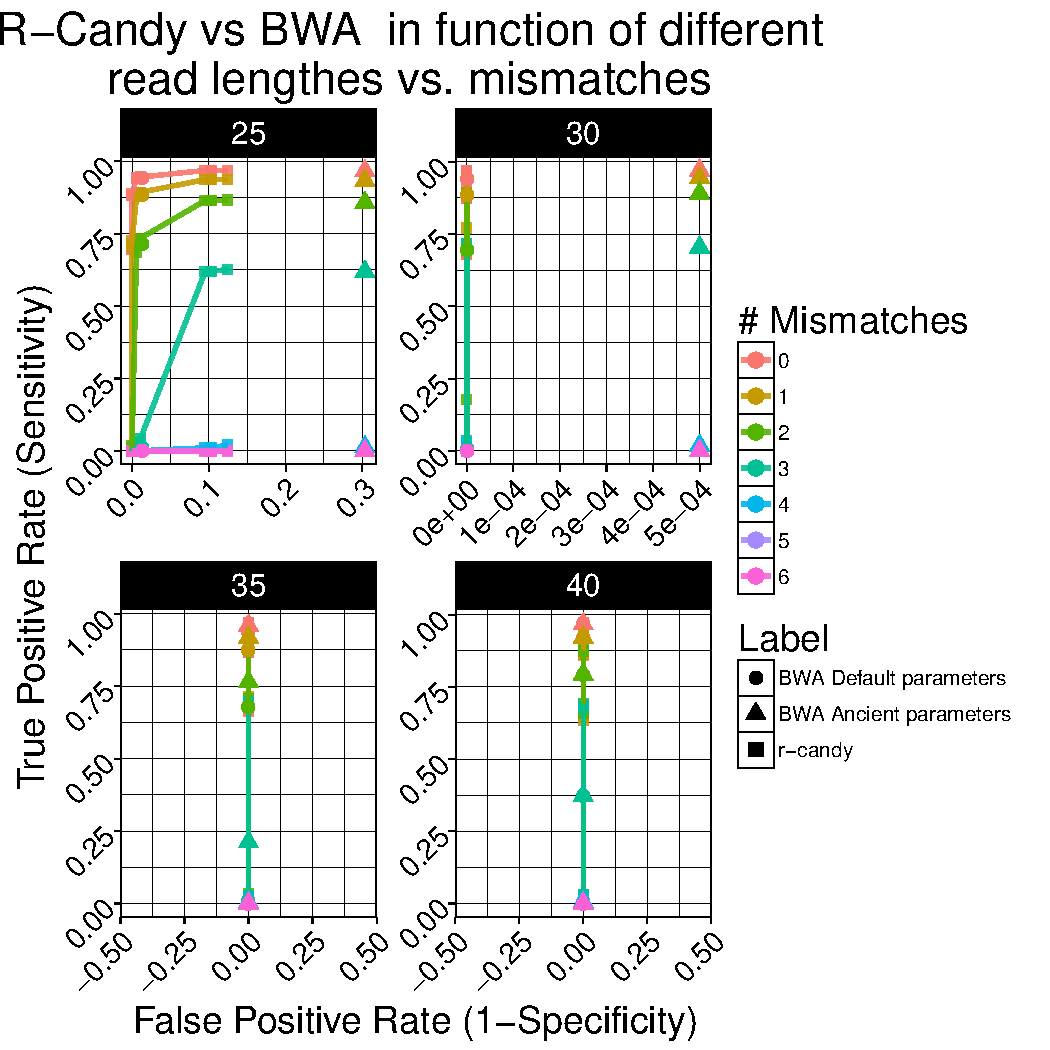
\includegraphics[width=12cm]{pictures/bROC_DS2_emp.pdf}
\caption{ROC curve for simulated reads with deamination damage and sequencing error by empirical quality distribution data, aligned to the simulated genome
         with true deamination parameters.}
\label{DS2_emp}
\end{figure}

\begin{figure}[H]
\centering
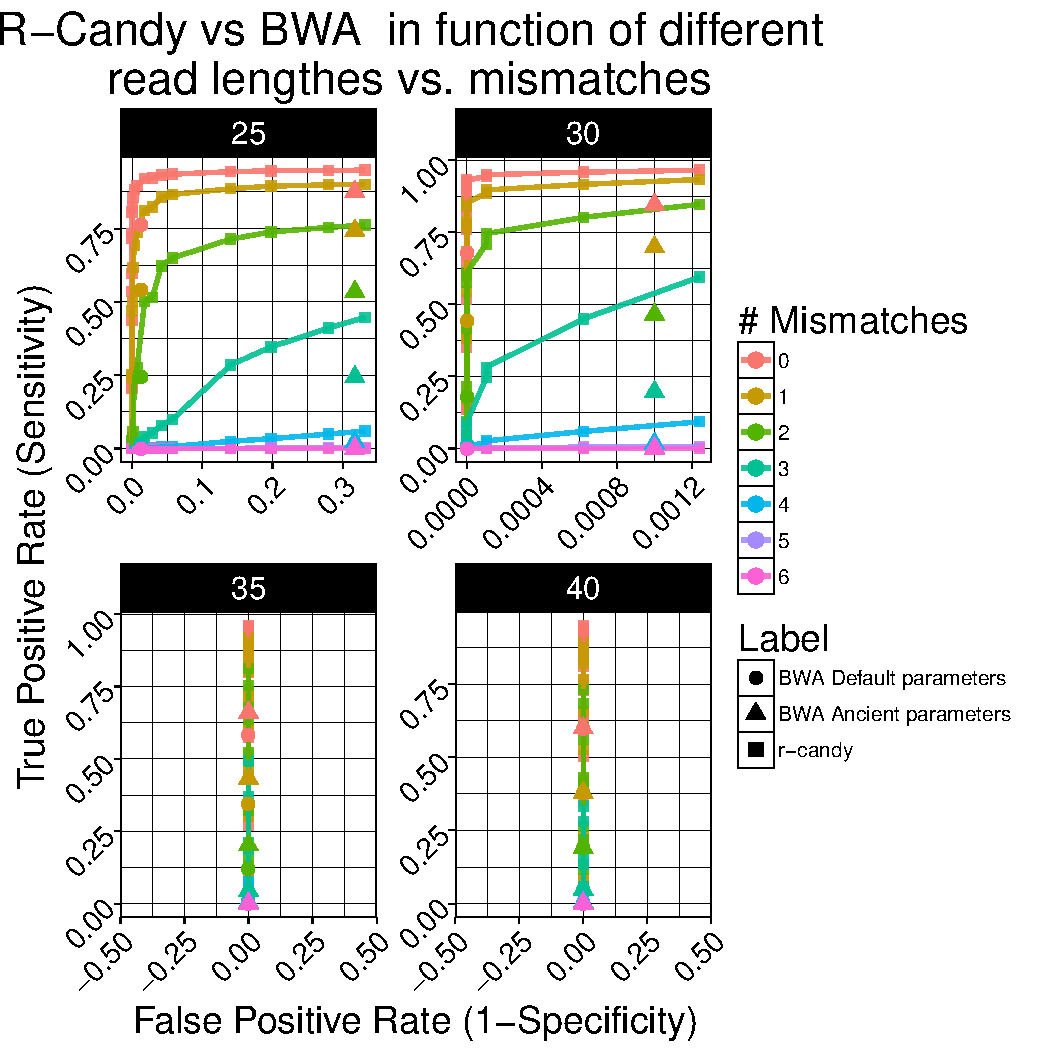
\includegraphics[width=12cm]{pictures/bROC_DS2_ART.pdf}
\caption{ROC curve for simulated reads with deamination damage and sequencing error for Illumina platform provided by ART aligned to the simulated genome
         with no deamination parameters.}
\label{DS2_ART}
\end{figure}

 
% \item Third, simulated reads with no deamination damage and align them to the simulated genome with R-Candy's default parameters and with actual parameters which are zero number for deamination parameters and also BWA with default and ancient parameters . 

\end{enumerate}





\begin{figure}[H]
\centering
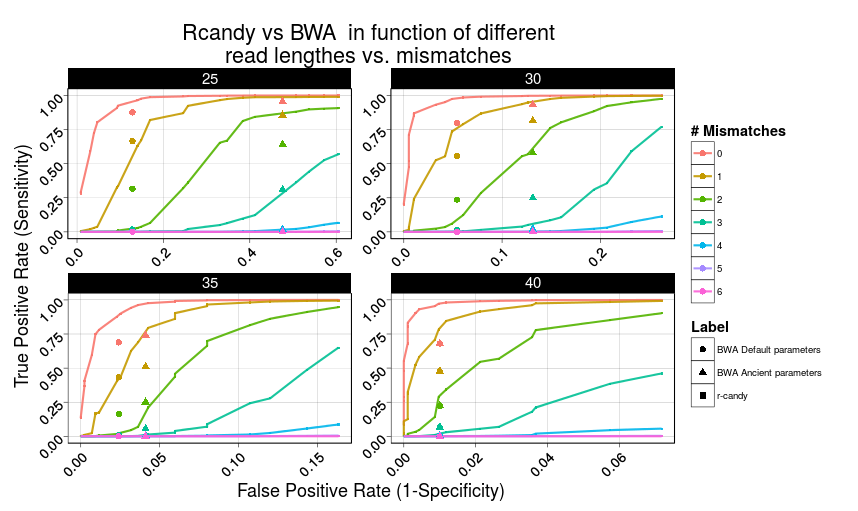
\includegraphics[width=12cm]{pictures/DS3-A.png}
\caption{ROC curve for simulated reads with sequencing error for Illumina platform provided by ART and no deamination damage aligned to the simulated genome.}
\label{DS3}
\end{figure}


\textbf{Discussion}


%%%%%%%%%%%%%%%%%%%%%%%%%%%%%%%%%%%%%%%%%%%%%%%%%%%%%%%%%%%%%%%%%%%%%%%%%

\subsection{Evaluation on Simulated Reads} 

The simulated reads are based on human genome 
 with introducing a different a small number of differences of $(0..6)$ and deamination based 
on Philip Jonson model parameters and also sequencing errors of Illumina empirical error profile.\\




%%%%%%%%%%%%%%%%%%%%%%%%%%%%%%%%%%%%%%%%%%%%%%%%%%%%%%%%%%%%%%%%%%%%%%%%%%%%%%
\subsubsection{Results} 

The same evaluation as Section 5.4.1 is done on simulated reads of real genome to see the effect of 
taking in account the deamination damage working with real genome. \\
Test data are:
\begin{itemize}

 \item Simulated reads with deamination and align to the human genome with R-Candy ran with 
the real deamination parameters (\emph{P}, $\delta$, $ \sigma $ and $ \sigma\prime $) and BWA with default
parameters ( no deamination parameters in BWA) and also BWA with ancient parameters (-n 0.01 , -o 2 ). 

 \item The same data aligned to R-Candy with no damage parameters. 
 
 \item Simulated reads with no deamination damage aligned to the human genome by R-Candy and BWA. 

\end{itemize}

\begin{figure}[H]
\centering
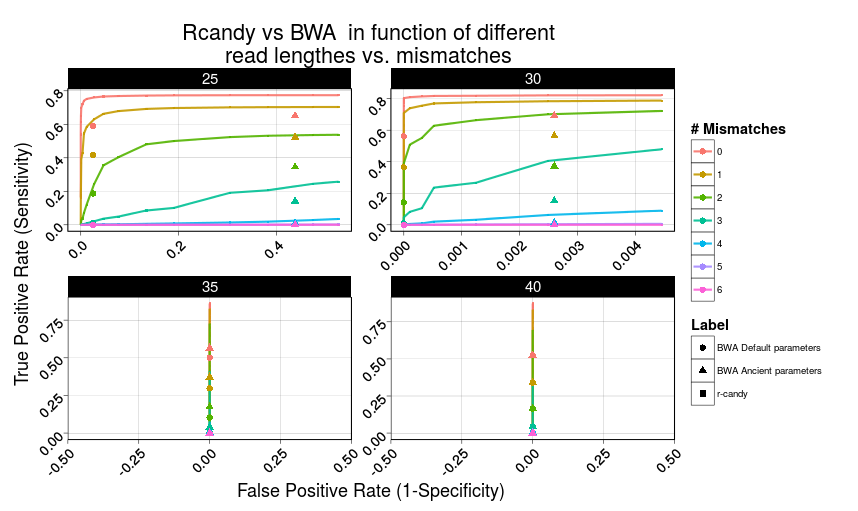
\includegraphics[width=12cm]{pictures/DS4.png}
\caption{ROC curve for simulated reads with deamination damage aligned to the human genome
         with deamination parameters.}
\label{DS4}
\end{figure}


\begin{figure}[H]
\centering
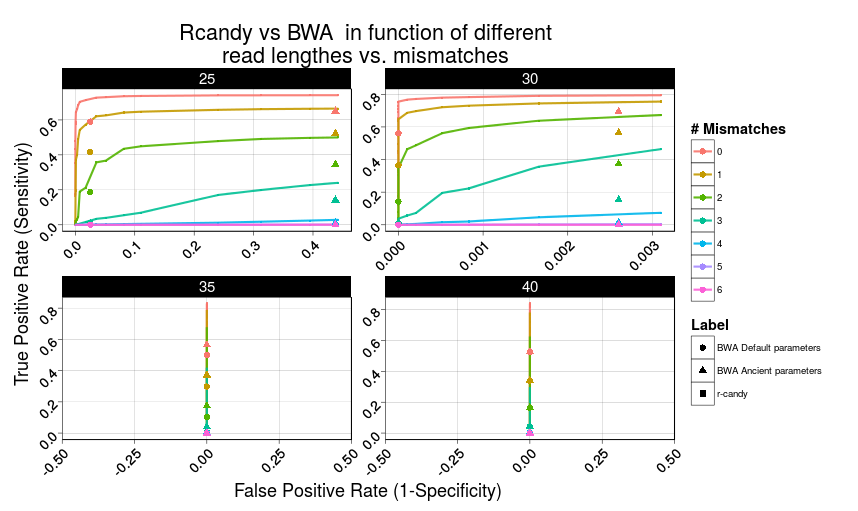
\includegraphics[width=12cm]{pictures/DS5.png}
\caption{ROC curve for simulated reads with deamination damage aligned to the human genome
         with no deamination parameters.}
\label{DS5}
\end{figure}

\begin{figure}[H]
\centering
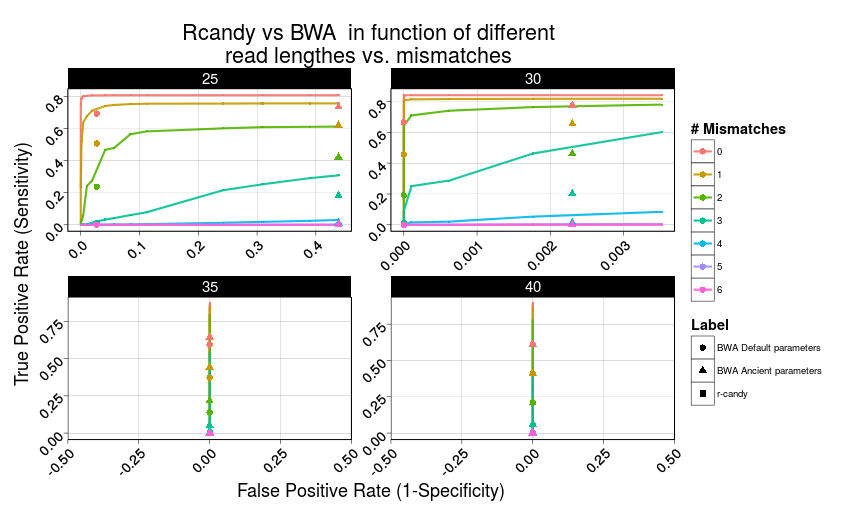
\includegraphics[width=12cm]{pictures/DS6.png}
\caption{ROC curve for simulated reads with no deamination damage aligned to the human genome.}
\label{DS6}
\end{figure}



%%%%%%%%%%%%%%%%%%%%%%%%%%%%%%%%%%%%%%%%%%%%%%%%%%%%%%%%%%%%%%%%%%%%%%%%%%%%%
%\subsection{Effect Of length on alignment}


%\subsection{Suitable alignment score}




%%%%%%%%%%%%%%%%%%%%%%%%%%%%%%%%%%%%%%%%%%%%%%%%%%%%%%%%%%%%%%%%%%%%%%%%%%%%
\section{Performance}

To evaluate R-Candy's speed, we used two test set, first simulated endogenous 
and microbial reads align to a simulated genome and second simulated endogenous
and microbial reads align to a real genome.\\

Tables  \ref{speed-SG} and \ref{speed-RG} show the running time of R-Candy on
a single CPU for the first and second test sets respectively.
Notice that the time required for building the R-Candy's index structure is 
not included in the reported running time.\\


As the results  show  the R-Candy's speed is affected by the read length on both cases.
It decreases from 0.123 number of aligned reads to the human genome per second for reads 
of length 25 bps to 0.045 number of aligned reads per second for reads of length 40 bps. \\
In both test sets, the longer the read is the more running time is required\\

On memory, R-Candy uses 2.5G for single-end mapping.\\

The current version of R-Candy does not support multi-threading to reduce the 
memory usage on multi-core computers.\\\\
We did not test R-Candy on real data because we do not know the ground truth
to help us on evaluating our software.\\
\begin{table}[H]
  \begin{tabular}{ |  p{2cm} | p{2cm} | p{3cm} | p{3cm} | p{3cm} |}
    \hline
  	\textbf{Type} & \textbf{Read length } &\textbf{Running time(s) } 
  	&\textbf{Speed \hspace{35pt}(no. of reads/s)} & \textbf{Speed \hspace{35pt}(no. of reads/s)}\\ \hline
  	  
 	  Genomic    & 25  & 74435.126s  & 0.134 \\ \hline
      Genomic    & 30  & 131637.035s & 0.075 \\ \hline
 	  Genomic	 & 35  & 150527.237s & 0.066 \\ \hline
 	  Genomic	 & 40  & 166909.584s & 0.059 \\ \hline
 	  Microbial  & 25  & 15676.300s  & 0.637 \\ \hline
      Microbial  & 30  & 20203.191s  & 0.494 \\ \hline
 	  Microbial  & 35  & 20932.235s  & 0.477 \\ \hline
 	  Microbial  & 40  & 22181.249s  & 0.450 \\ \hline
 	  
   \end{tabular}
\caption{The R-Candy alignment speed for bacterial reads aligned to the human reference genome}
\label{speed-SG}
\end{table}



\begin{table}[h]
  \begin{tabular}{ |  p{2cm} | p{2cm} | p{3cm} | p{3cm} | }
    \hline
  	\textbf{Type} & \textbf{Read length } &\textbf{Running time(s) } &\textbf
     {Speed\hspace{35pt}(no. of reads/s)} \\ \hline 
  
      Genomic   & 25  & 80816.842s   & 0.123 \\ \hline
      Genomic   & 30  & 1377473.004s & 0.007 \\ \hline
 	  Genomic	& 35  & 209116.332s  & 0.047 \\ \hline
 	  Genomic	& 40  & 219178.156s  & 0.045 \\ \hline
 	  Microbial & 25  & 18490.615s   & 0.540 \\ \hline
      Microbial & 30  & 31276.839s   & 0.319 \\ \hline
 	  Microbial & 35  & 34546.643s   & 0.289 \\ \hline
 	  Microbial & 40  & 33363.229s   & 0.299 \\ \hline
 	  
   \end{tabular}
\caption{The R-Candy alignment speed for simulated reads aligned to the human reference genome}
\label{speed-RG}
\end{table}



%%%%%%%%%%%%%%%%%%%%%%%%%%%%%%%%%%%%%%%%%%%%%%%%%%%%%%%%%%%%%%%%%%%%%

\section{Conclusions}


%%%%%%%%%%%%%%%%%%%%%%%%%%%%%%%%%%%%%%%%%%%%%%%%%%%%%%%%%%%%%%%%%%%%%%
\section{Future Work}
Use dynamic programming (DP) for alignment algorithm and implement it in the way that instead of filling 
\emph{score matrix} in a rectangular stick with some diagonals if we know that we will have more match/mismatch instead of INDELs.
And also, using seed strategy which needs to sub-divide the alignment and start from different places.
But we need a \emph{Bidirectional Wavelet Tree}\cite{bidirectional} for that. Start aligning from the middle 
of the reads (because that is the best part that we have in ancient DNA) in one direction and then the other direction, 
we need a Bidirectional Wavelet Tree to turn around.



%%%%%%%%%%%%%%%%%%%%%%%%%%%%%%%%%%%%%%%%%%%%%%%%%%%%%%%%%%%%%%%%%%%%%%
\section{Availability}

R-Candy's documentation and source code are freely available at:\\
 (https://github.com/udo-stenzel/r-candy.git).
\\

Genome/read simulation program written in C++ is freely available at\\ 
(https://github.com/Homa1127/simulateGenome.git).


The hash program for analysing  R-Candy's output written in C++, available at: \\
https://github.com/Homa1127/rcandyHash.git

%%%%%%%%%%%%%%%%%%%%%%%%%%%%%%%%%%%%%%%%%%%%%%%%%%%%%%%%%%%%%%%%%%%%%%%%

\section{Abbreviations}

DNA: deoxyribonucleic acid;
bp: base pair;
NGS: next generation sequencing technologies;
BWT: Burrows-Wheeler transform;
FM: full-text minute-space;
A: Adenine;
C: Cytosine;
T: Thymine;
G: Guanine;
PacBio: Pacific Bioscience;
SA: suffix array;
LF: last to first;
DFS: depth first search;
DP: dynamic programming;
BAM: Binary Alignment/Map;
CDF: cumulative distribution function.
PCR: Polymerase Chain Reaction.
%%%%%%%%%%%%%%%%%%%%%%%%%%%%%%%%%%%%%%%%%%%%%%%%%%%%%%%%%%%%%%%%%%%%%


\bibliographystyle{unsrt}
\bibliography{Ref}


\end{document} 
   
      
      
              
